% RECOMMENDED %%%%%%%%%%%%%%%%%%%%%%%%%%%%%%%%%%%%%%%%%%%%%%%%%%%
\documentclass[graybox]{svmult}
\usepackage[hyperfootnotes=false]{hyperref}
\hypersetup{bookmarksdepth=3}
% choose options for [] as required from the list
% in the Reference Guide

\usepackage{mathptmx}       % selects Times Roman as basic font
\usepackage{helvet}         % selects Helvetica as sans-serif font
\usepackage{courier}        % selects Courier as typewriter font
\usepackage{type1cm}        % activate if the above 3 fonts are
                            % not available on your system
%
\usepackage{makeidx}         % allows index generation
\usepackage{graphicx}        % standard LaTeX graphics tool
                             % when including figure files
\usepackage{multicol}        % used for the two-column index
\usepackage[bottom]{footmisc}% places footnotes at page bottom
%\documentclass{article}
% \usepackage{tikz}
 \usepackage{adjustbox}
 \usepackage{multirow}
 \usepackage{algorithm}
 \usepackage{algpseudocode}
 \usepackage{ifthen}
 %\usepackage{csquotes}
 \usepackage{amsmath}
\newboolean{enable-backrefs} % enable backrefs in the bibliography
\setboolean{enable-backrefs}{true} % true false
\newcommand{\backrefnotcitedstring}{\relax}%(Not cited.)
\newcommand{\backrefcitedsinglestring}[1]{(Cited on page~#1.)}
\newcommand{\backrefcitedmultistring}[1]{(Cited on pages~#1.)}
\ifthenelse{\boolean{enable-backrefs}}%
{%
		\PassOptionsToPackage{hyperpageref}{backref}
		\usepackage{backref} % to be loaded after hyperref package
		   \renewcommand{\backreftwosep}{ and~} % separate 2 pages
		   \renewcommand{\backreflastsep}{, and~} % separate last of longer list
		   \renewcommand*{\backref}[1]{}  % disable standard
		   \renewcommand*{\backrefalt}[4]{% detailed backref
		      \ifcase #1 %
		         \backrefnotcitedstring%
		      \or%
		         \backrefcitedsinglestring{#2}%
		      \else%
		         \backrefcitedmultistring{#2}%
		      \fi}%
}{\relax}
\usepackage{comment}
 \usepackage{natbib}
 \setcitestyle{authoryear,round,aysep={,}}
% \usepackage{hyperref}
 \usepackage{graphicx}
 \usepackage[subrefformat=parens,labelformat=simple,caption=false,labelfont={bf}]{subfig}
 \usepackage[nolist,smaller]{acronym}
 \usepackage{sidecap}
% \usepackage{nomencl}

\makeindex

\begin{document}
\begin{acronym}[ALSPAC]
  \acro{FAS}{Foetal Alcohol Syndrome}
  \acro{CPT}{Cumulative Prospect Theory}
  \acro{PT}{Prospect Theory}
  \acro{NICE}{National Institute for Health and Care Excellence}
  \acro{IAPT}{Improving Access to Psychological Therapies}
  \acro{CMACE}{Centre for Maternal and Child Enquiries}
  \acroindefinite{CMACE}{the}{the}
  \acro{AUDIT}{Alcohol Use Disorders Identification Test}
  \acro{T-ACE}{Tolerance, Annoyance, Cut down, Eye-opener}
  \acro{RCOG}{Royal College of Obstetricians and Gynecologists}
  \acroindefinite{RCOG}{the}{the}
  \acro{AML}{acute myeloid leukemia}
  \acro{ADHD}{Attention Defecit Hyperactivity Disorder}
  \acro{PND}{Postnatal Depression}
  \acro{RCT}{randomised control trial}
  \acro{WHO}{the World Health Organisation}
  \acro{ESS}{Evolutionarily Stable Strategy}
  \acrodefplural{ESS}[ESS]{Evolutionarily Stable Strategies}
  \acro{MCMC}{Markov chain monte carlo methods}
  \acro{DU}{Discounted Utility}
  \acro{AIC}{Akaike information criterion}
  \acro{ANOVA}{analysis of variance}
  \acro{ALSPAC}{the Avon Longitudinal Study of Parents and Children}
  \acro{GEM}{Gaussian Emulation Machine}
  \acrodefplural{GEM}{Gaussian Emulation Machines}
  \acro{GEM-SA}{Gaussian Emulation Machine for Sensitivity Analysis}
  \acro{JIT}{Just-in-time}
  \acro{ABM}{Agent Based Modelling}
  \acro{ABMs}{Agent Based Models}
  \acro{CPT}{Cumulative Prospect Theory}
  \acro{FFH}{Fast and Frugal Heuristic}
  \acro{OFC}{orbito-frontal cortex}
  \acro{BACCO}{Bayesian Analysis of Computer Code Outputs}
  \acro{IQR}{interquartile range}
\end{acronym} 

\title*{Deciding to Disclose}
\subtitle{A Decision Theoretic Agent Model of Pregnancy and Alcohol Misuse}

\author{Jonathan Gray, Jakub Bijak, and Seth Bullock}
% Use \authorrunning{Short Title} for an abbreviated version of
% your contribution title if the original one is too long
\institute{Jonathan Gray \at University of Southampton, Southampton, United Kingdom \email{j.gray@soton.ac.uk}
\and Jakub Bijak \at University of Southampton, Southampton, United Kingdom \email{j.bijak@soton.ac.uk}
\and Seth Bullock \at University of Southampton, Southampton, United Kingdom \email{sgb@ecs.soton.ac.uk}}

\maketitle

%*************************
% Acronyms
%*************************
%\phantomsection
%\refstepcounter{dummy}
%\pdfbookmark[1]{Acronyms}{acronyms}
%\markboth{\spacedlowsmallcaps{Acronyms}}{\spacedlowsmallcaps{Acronyms}}
%\section*{Acronyms}
             
%\refstepcounter{dummy}
%\pdfbookmark[1]{Glossary}{glossary}
%\printglossary[type=main]

%\printnomenclature{}

%Assuming this is for JASSS.. Need to make background shorter.
%Aim for ~ 7-8,000 words overall.

\begingroup
\let\clearpage\relax
\let\cleardoublepage\relax

\pdfbookmark[1]{Abstract}{Abstract}


\section*{Abstract}

Background: 

Objective: 

Methods: 

Results: 

Conclusions:

Comments: 

This dissertation presents a method for modelling disclosure behaviour
by treating the interaction as paired signalling games played by decision
theoretic agents. Two theories of decision making - Bayesian risk
minimisation, and \ac{CPT} - are investigated, and a simulation developed
using Python.

The feasibility of the method is examined through a case study, which
considers the disclosure of the drinking behaviour of pregnant women
to their midwives. 

The essence of the scenario is that there is considered to be a long
term benefit to disclosure - common in the healthcare arena, but an
opportunity cost associated with disclosure. In the case study, this
is conceptualised as arising from the perceived undesirability of
drinking while pregnant. More generally this could derive from any
imbalance in the long term benefit and the opportunity cost, for example
the subjective benefit of a cigarette in the near future, versus the
discounted benefit of better health later.

Theories of decision are driven by the weighing of probabilities and
subjective gains or losses. In this case, the probabilities are generated
by individual agents based on their initial preconceptions and their
experiences across the simulation, using Bayesian inference.

The Bayesian risk minimising model is able to reproduce qualitative
trends around increased honesty over appointments, and a negative
impact of harsh judgement of drinkers on disclosure. The \ac{CPT}
model is less successful, which may be a result of improper, or excessively
homogenous parameters, in combination with unrealistic payoffs.

A global sensitivity analysis is also conducted using Gaussian Emulation
Machines, and finally recommendations for further work are dervived, along
with a few key recommendations for practice - assume people are being honest,
and be non-judgemental.

\vfill{}


\endgroup


\acresetall

%!TEX root = disclosure_game.tex
\section{Introduction}
\label{sec:intro}
%CONTRIBUTION, FUCKER!
%Also, remember to say what you're going to do for the rest of the article?
%CONTRIBUTION
%	Agents are awesome
%	Decision theory is super awesome
%	'nice story to hang it on'
% 	mention the importance of behaviour change
% tool for thinking
% theoretical vacuum at the middle
% under what scenarios does an as if explanation break down

The case in favour of \ac{ABM} as a general analytical approach has been made numerously, and elegantly (e.g. \citet{epstein1994growing,Resnick,Axelrod1997,gilbert1999simulation,Macy2002a,Silverman2011,Silverman2013,epstein2014agent_zero}, amongst others). As such we will not belabour the point, and instead turn to addressing some of the concerns expressed about the approach. In this instance we focus on the perception of \ac{ABM} as ad hoc in nature, tending to be a reflection of the assumptions of the modeller rather than empirically or theoretically grounded \citep{Waldherr2013}. To ameliorate this concern, we draw on decision theory to produce simple rule based, learning, decision making agents and show that they are able to play a form of signalling game\footnote{In a signalling game, on player, the signaller, has some piece of information that is known only to them which affects the outcome of the game for both players. The signaller has a choice as to what they tell the other player about this hidden information, and the responding player as to what they believe the information to be.} \citep{Kreps1987} with a basic form of intragroup information sharing. Four decision models of varying complexity, and behavioural plausibility are contrasted, by way of demonstrating the significance of the operationalisation of decision making in \ac{ABM}.

This exercise is framed in the context of disclosure decisions, taking drinking patterns in pregnant women as a motivating example. Alcohol consumption in the antenatal period is a significant issue in itself, and has been associated with many potentially negative consequences. For example, \citet{Andersen2012} report results from a large scale Danish cohort study suggesting that even low levels of consumption in early pregnancy increase the risk of spontaneous abortion, although \citet{Savitz2012} has suggested this may be attributable to a previously known link to absence of mornining sickness. Risk continues to the point of birth - \citet{Kesmodel2002} found a heightened risk to the infant - into childhood, with a metastudy by \citet{Latino-Martel2010} finding evidence on an increased risk of childhood \ac{AML}. Harm may also extend even further, and a review by \citet{Huizink2006} concluded that maternal alcohol consumption could be a contributing factor to \ac{ADHD}, and other learning impairments, but note methodological issues in a number of the papers. There is not, however, a clear consensus, with \citet{Gray2006} finding no evidence of harm below 1.5 UK units\footnote{Roughly half a pint of beer, a single 25ml measure of spirits, or one 175ml glass of wine.} per day. In terms of official guidance in the UK, \ac{NICE} acknowledge that evidence of harm to the fetus is less than conclusive, but advise not drinking at all, or significant moderation \citep{NICE2010a}, with similar advice from the UK \cite{DepartmentofHealth2008}.

Turning more specifically to disclosure of alcohol use by women during their pregnancy, research is relatively sparse, although qualitative trends are reported by \citet{Phillips2007} and \citet{Alvik2006}. The former explored factors impacting disclosure through a small case study, highlighting the need to build up rapport between woman and midwife over several appointments; the latter compared post partum reports of consumption with contemporaneous accounts, finding apparent underreporting during pregnancy which was amplified by increased drinking. The simulation model described in this paper is able to replicate both qualitative trends, i.e. an increase in disclosure over appointments, and more honest behaviour by moderate as compared to heavier drinkers.

The resulting scenario is of substantial independent interest, and shows the potential utility of a simulation approach in arenas where randomized control trials are not viable for ethical, or financial reasons. With this said, the lack of a strong quantitative evidence base against which to validate the behaviour of the model augers for caution in interpreting the results, and a necessary reminder that in this instance the model is primarily a tool for formalisation of the thought process \citep{epstein2008}, rather than a machine for predicting.

%two fold appeal. cognitive plausibility - neuroec. inaccessible systems (litigation, concealment). fast. cheap. portable. theoretical grounding. rigor.

A game theoretic approach to generating an abstract form of the problem gives a convenient, and well known framework to reason about the processes involved in the scenario. While scenarios may map to a number of games, exploring one candidate game still allows for a principled comparison between interpretations, and enforces explicit assumptions. Relating this to decision theory shifts the emphasis away from analytical equilibrium-seeking, and heightens the importance of behaviour change. This is clearly desirable where the focus is on the behavioural processes driving a system in motion, and how they change in response to that movement.
Fundamentally, the shift of emphasis is from the process of acquiring and inferring the information needed to make choices, to the process of decision.
Naturally, this does not preclude the incorporation of strategic refinement, since decision rules are to a great extent modular, and as demonstrated in this paper can be exchanged without altering the underpinning decision problem. In addition, rules are agnostic as to where the information used derives from, suggesting room for multi-stage processes.  As a corollary, the decision problem agents attempt to answer can change, allowing agents' behaviour in novel problems to be informed by beliefs derived under other conditions. 

While there is no universal theory of human behaviour to sit at the centre of \ac{ABM}ing as a method, a key motivation for decision rules is their claim to provide an account of decision making that is behaviourally and cognitively plausible. Their mooted capability in this regard is to some extent supported by work from neuroeconomics, which aims to empirically test theories of decision making \citep{Rustichini2009}. Many key aspects common to decision rules, for example the idea that a common currency is used by the brain to compare outcomes \citep{Padoa-Schioppa2006,Padoa-Schioppa2008}, are supported by neurological findings. In addition, a single decision rule represents a pleasingly parsimonious alternative to numerous case specific production rules. 

Given these features, the application of decision, and game theory to \ac{ABM} is an attractive approach to computational social science, where the locus of interest is decision making. Taking a balance between models focused on replication of low level neurological mechanics, and those with a higher level emphasis where individual behaviours are abstracted away yields a computationally tractable approach. Despite the relative simplicity, it nonetheless captures some of the nuance and sophistication of human decisions.

%Finishing up

The remainder of this paper proceeds to provide a brief review of the methodological context (section \ref{sec:lit_review}), before outlining the model (section \ref{sec:model}), and experiments (section \ref{sec:method}), with selected results (section \ref{sec:results}), followed by a discussion contrasting the decision models (section \ref{sec:discussion}), and conclusions (section \ref{sec:conclusion}). %(half page)

%!TEX root = disclosure_game.tex
%Rewrite all of this, ditch the alcohol stuff altogether. Any really key can be woven in elsewhere (discussion)
\section{Previous Research}

\label{sec:lit_review}

This section presents a brief overview of previous research, addressing in turn signalling games, normative decision theory, heuristic decision making, and descriptive decision theory.


\subsection{Signalling Games}

The majority of classical game theory focuses on strategic decision making, in scenarios where all players have complete information about all aspects of the game. An alternative, perhaps more common situation, is that players have incomplete information, i.e. their knowledge of the state of the world is in some way deficient. \citet{Harsanyi1967} introduced the concept of a Bayesian game, resolving the problems introduced by the incomplete information scenario by allowing the possible variations on the rules to be treated as subgames. This adds an additional player - nature, to the game, where nature takes the first move thereby deciding which subgame is played. Nature is assumed to make their move by lottery, and where the probability distribution governing the lottery is known to all players this permits the game to be formulated as one of complete information. 

Here, we are specifically interested in signalling games \citep{Kreps1987,Spence1973}, where one player holds some private information which may be communicated (or not) by means of a signal.
This basic form has been widely applied, with substantial interest in what conditions permit honest signalling as Nash equilibria or \acp{ESS}. \citet{Grafen1990}, following from a suggestion by \citet{Zahavi1975}, proposed that if signals intended to indicate mate quality exacted a cost on the signaller (e.g. peacock tail feathers), then honest signalling would constitute an \ac{ESS}. Similar results have also been demonstrated in a game of job market signalling, where signal cost was differentiated by type \citep{Spence1973}. 
Costly signalling has also been suggested as an explaination of behaviour that at first glance appears counter intuitive, for example \citet{Godfray1991} applied the idea to the food solicitation behaviour of chicks, where a stronger signal carries a risk of being eaten. Moving beyond animal behaviour, \citet{Sosis2003} considered the implications of ritual behaviour, in the context of religion, represented a costly signal, an idea subsequently extended by \citet{Henrich2009} to include cultural transmission, and \citet{Wildman2011} to introduce group differentiation.

Other work augments the signalling game model, for example \citet{Austen-Smith2005} add a second `peer group' audience signalling game to the original \citeauthor{Spence1973} game in an effort to explain poor academic performance in some social groups, with some subseqent empirical support for the idea from \citet{Jr2010}. On a similar tack, \citet{Feltovich2002} introduce additional noisy type information, finding that this effectively explained counterintuitive observed behaviour where actors with every right to boast of their quality fail to do so.

\subsection{Normative Decision Theory}

While game theory addresses rational strategic decision making, decision theory deals instead with rational decision making \citep{Peterson2009}.  Taken literally, this leads to normative decision theory, where the focus is on giving the rational answer to a decision problem. An alternative view - descriptive, or behavioural decision theory, holds that the focus should instead be on giving an account of human decision making performance, complete with observed deviations from perfect rationality, which we address in section \ref{sub:descriptive_theories}. Finally a third perspective, which to some extent overlaps this division, suggests that decisions are heuristic in nature and rational in ecological context \citep{Gigerenzer1996} (section \ref{sub:heuristic_theories}).

The conceptual underpinning of all of these is the central idea of expected utility, originated by \citet{Bernoulli1954} and later formalised by \citet{Neumann1953}, which treats all decisions as gambles defined in terms of payoffs and probabilities.

Recently, several studies have explored biological correlates to aspects of expected utility. The fundamental concept, that all outcomes are comparable in a universal currency has been supported by evidence of neural correlates of decision variables \citep{Platt1999}, and following from this results from \citet{Padoa-Schioppa2006,Padoa-Schioppa2008} showing neuronal firing in the \ac{OFC} corresponding to revealed preferences in monkeys. Additionally, some support for neural representation of value, and risk aversion was found by \citet{Christopoulos2009}. The model presented in this paper makes an explicit assumption that social decisions utilise the same process, and while this is less well supported there is some evidence to suggest involvement by the same brain region, since damage to the \ac{OFC} has been shown to impair social judgements in both primates \citep{Watson2012}, and humans \citep{Willis2010}.

An alternative normative model of decision making is Bayesian decision theory, proposed by \citet{Robbins1964}, which is essentially the application of Bayesian style probabilities to the expected utility model. This allows probabilities used in reasoning to be subjective, which may allow for a better account of decisions from experience (see \citet{Hau2008,Hertwig2004} for results elucidating the distinction, and comparing the performance of several non-Bayesian models). This model has seen notable successes in practical problems \citep{McNamara1980,Survey2003,Kristensen1997}, but suggestions by several authors  that it could constitute an effective (top-down) model of learning \citep{Tenenbaum2006,Griffiths2010}, or induction \citep{Gallistel2012} in the brain have attracted substantial criticism\footnote{For example \citet{Bowers2012} responding to \citet{Tenenbaum2006}, and \citet{Griffiths2010}; and \citet{Miller2012} addressing \citet{Gallistel2012}.}.

\subsection{Heuristic Decision Making}\label{sub:heuristic_theories}

As noted, heuristic decision making stems from a contention that \citeauthor{Neumann1953} type rationality ignores the context of decision making, and a lack of correspondence between predicted and actual human decisions (see, for example the Allais paradox \citep{Society2013}, and subsequent empirical support \citep{Oliver2003,Burke1996}). Arguably, this notion begins with \citet{Simon1956}, who suggested that humans do not attempt to make optimal choices, but to satisfice and choose the first `good enough' option. While noting that this will often achieve the same result, the claim is that humans exhibit bounded rationality \citep{Simon2000} arising from inherent limits to cognition.

\citet{Gigerenzer1996} take the concept of bounded rationality further, and argue for what they term \acp{FFH}. This recasts rationality as bound to the context of the behaviour: a rational approach to choosing the right mate might well require checking every possible partner, but given finite time, memory, and so on rapidly becomes unachievable. On this basis, they contend that the rationality of any given decision rule can only be determined in the context of the environment \citep{Todd2003}, which implies that heuristics are task specific. They provide a number of heuristics for varying decision problems, e.g. recognition \citep{Goldstein2002}, cue ordering \citep{Gigerenzer1999,Todd2004}, and binary decisions \citep{Brandstatter2006}.

\subsection{Descriptive Decision Theory}\label{sub:descriptive_theories}

While heuristic theories arguably fall under the purview of the descriptive, the wider tendency is towards what are in essence \enquote{patches} to normative models. The most influential models in this class derive from \ac{PT} \citep{Kahneman1979}, which combines a set of heuristics based on observed decision behaviour \citep{Tversky1974}, with distortions to the perception of probability, and the value of outcomes \citep{Kahneman1984,Tversky1986}. \citet{Tversky1992} subsequently addressed issues present in their original formulation by introducing \ac{CPT}, which allows for non-binary decisions, but dispenses with the heuristic aspects of the original formulation. The essence then, is that high and low probabilities are treated differently, and the subjective value of a loss differs from the equivalent gain (losing your shirt is perceived as more of a loss than winning a shirt is a gain).
This last effect, known as the framing effect is particularly significant, see for example work by \citet{Toll2007} examining the relationship between loss and gain framings and success rates in giving up smoking, and \ac{NICE} guidance on framing of treatment options \citep{NICE2007}.

\ac{CPT} has been successful in explaining a number of anomalous results in decision tasks (see \citet{Camerer2004a} for a review), and \citet{Thaler2000} comments to the effect that the theory is promising, albeit incomplete, lacking for example any explanation of how frames are constructed. While remaining an effective account of decision behaviour under risk, the theory does not attempt to resolve apparent inconsistencies that arise when outcomes are delayed, i.e. in situations of intertemporal choice. Historically, \ac{DU} \citep{Samuelson1937}, which effectively claims that the value of a thing now is exponentially greater than the promise of the same thing at some future date, has been applied to explain this. More recently, \citet{Ainslie1991} has suggested that discounting of future outcomes is hyperbolic, rather than exponential. However neither model is complete, in that both fail to account for results from \citet{Thaler1981} showing differing temporal discounting rates for losses and gains. \citet{Loewenstein1992} report additional failings in classic \ac{DU} models, and propose a modified form of \ac{CPT} which they suggest is able to handle both immediate, and intertemporal choice.

%!TEX root = disclosure_game.tex
\section{Disclosure Game Model}
\label{sec:model}
%Start this off with a brief description of our fictional scenario.
% Whole section ~ 1.5K

In this section we outline the disclosure game model, and give details of the four decision rules that will be examined in this paper, but begin with a brief sketch of a pregnancy in terms of encounters between a pregnant woman and a midwife. 

Typically in the UK, a women will have 12 appointments with a midwife during the antenatal period, and in the majority of cases will encounter several different midwives \citep{Redshaw2014} in the course of their care. In the UK, and unlike most healthcare scenarios, maternity notes are held by the patient, so midwives do not have extensive information prior to an appointment unless they have encountered the woman previously. Maternity notes are not generally linked to extra-departmental records, meaning that a history of alcohol related admissions to another service may remain unknown unless revealed by the woman.

According to NICE guidance \citep{NICE2010a,NICE2010} the issue of substance misuse should be raised at the initial booking appointment, followed by subsequent action if a concern is raised is at the discretion of the midwife. This may take the form of specific guidance to reduce intake, or if deemed necessary a referral to a specialist midwife and relevant interdisciplinary team. On alcohol consumption, policy regarding how to determine the level of consumption is at the time of writing generally at the level of local health authority, hospital trust, or according to the best judgement of the individual midwife, with no guidance provided by NICE. This commonly takes the form of average units per week, but may include \ac{T-ACE}\footnote{The \ac{T-ACE} is a four question screening test for alcohol misuse intended specifically for use with pregnant women.} \citep{Sokol1989863} and similar measures. 

Beyond the \enquote{booking} appointment, the onus is on women to raise concerns about their drinking behaviour, or the midwife to probe further if they feel it is warranted. In either case, once a concern has been raised the midwife must respond clinically, and inevitably personally, to the information.

In an ideal world, all interactions with healthcare providers would be immediately and fully disclosive, with no repercussions for the patient. However, alcohol misuse by women is known to attract stigma \citep{Gomberg1988}, and is a recognised barrier to appropriate treatment in the maternity context \citep{NICE2010,Radcliffe2011}.

\subsection{Disclosure Game}
\label{sub:the_game}
%Outline how the scenario translates into a game.
%Brief mention of the game theoretic solution

In order to translate the scenario sketched above into a more abstract, tractable form, we cast it as a signalling game, and assume that women's disclosures (or not), are signals. We also make the simplifying assumption that a woman may have one of only three drinking patterns - light\footnote{Or abstinent, the extent of alcohol consumption being such that it would generally be felt to pose essentially no risk.}, moderate, or heavy. Correspondingly, they are limited in what signals they may send when claiming to be one of these three types. 

Midwives are treated in a similar fashion, where their type corresponds to how negatively they regard a drinking pattern - non-judgemental, moderately judgemental, and harshly judgemental. The expression of this judgement is not a matter of choice on their part, and is assumed to have no impact on their clinical response, which is to either refer the woman for specialist treatment, or do nothing.

At the end of a game, each player receives a payoff dependent on the actions and types of both players. Because both women and midwives have an interest in the outcome of the pregnancy, and would prefer a healthy baby, the payoff has a common interest component. Hence, both players receive a payoff based on the health of their eventual baby, but women bear a social cost dependent on the signal they sent and the midwife's reaction to it. Similarly, midwives pay a cost if they refer to a specialist, mirroring the organisational cost of non-routine care. Table \ref{tab:Payoff-matrix} shows the three payoff matrices which together describe the game.

\begin{table}
\center
\subfloat[Social cost, \(X_{s}\), for women, given their signal, and the midwife's type\label{tab:Social-cost-matrix}]{%
\begin{tabular}{|c|c|c|c|c|}
\cline{3-5} 
\multicolumn{2}{c}{} & \multicolumn{3}{|c|}{Woman}\tabularnewline

\hline
\multirow{4}{*}{\rotatebox[origin=c]{90}{Midwife}} &  & Heavy & Moderate & Light\tabularnewline
\cline{2-5} 
 & Harsh & -2 & -1 & 0\tabularnewline
\cline{2-5} 
 & Moderate & -1 & 0 & 0\tabularnewline
\cline{2-5} 
 & Non & 0 & 0 & 0\tabularnewline
\hline 
\end{tabular}

}

\subfloat[Health outcome, \(X_{h}\), for women and midwives, given the midwife's action, and woman's type\label{tab:Referral-payoff-matrix}]{%
\begin{tabular}{|c|c|c|c|c|}
\cline{3-5} 
\multicolumn{2}{c}{} & \multicolumn{3}{|c|}{Woman}\tabularnewline

\hline 
\multirow{3}{*}{\rotatebox[origin=c]{90}{Midwife}} &  & Heavy & Moderate & Light\tabularnewline
\cline{2-5} 
 & Refer & 10 & 10 & 10\tabularnewline
\cline{2-5} 
 & Don't refer & -2 & -1 & 10\tabularnewline
\hline 
\end{tabular}

}

\subfloat[Referral cost, \(X_{c}\), for midwife, given their action and the woman's type\label{tab:inst_cost_matrix}]{%
\begin{tabular}{|c|c|c|c|c|}
\cline{3-5}  
\multicolumn{2}{c}{} & \multicolumn{3}{|c|}{Woman}\tabularnewline
\hline 
\multirow{3}{*}{\rotatebox[origin=c]{90}{Midwife}} &  & Heavy & Moderate & Light\tabularnewline
\cline{2-5} 
 & Refer & -9 & -9 & -9 \tabularnewline
\cline{2-5} 
 & Don't refer & 0 & 0 & 0\tabularnewline
\hline 
\end{tabular}

}

\caption{Payoff matrices\label{tab:Payoff-matrix}}
\end{table}

Taken together, this leads to a game tree that is relatively complex (figure \ref{fig:simple_tree} shows a simplified representation, with a detailed view of one branch in figure \ref{fig:zoom_tree}) even at the subgame level. Rather than attempt to solve for equilibria, agents treat this two player game as taking place against nature, along the lines of adversarial risk analysis \citep{RiosInsua2009}. This effectively translates the game to a pair of decision problems (figure \ref{fig:decision_problems}), which agents attempt to resolve at each turn using a simple decision rule, given their prior beliefs and experience of play.

\begin{figure}[H]
\begin{adjustbox}{center}
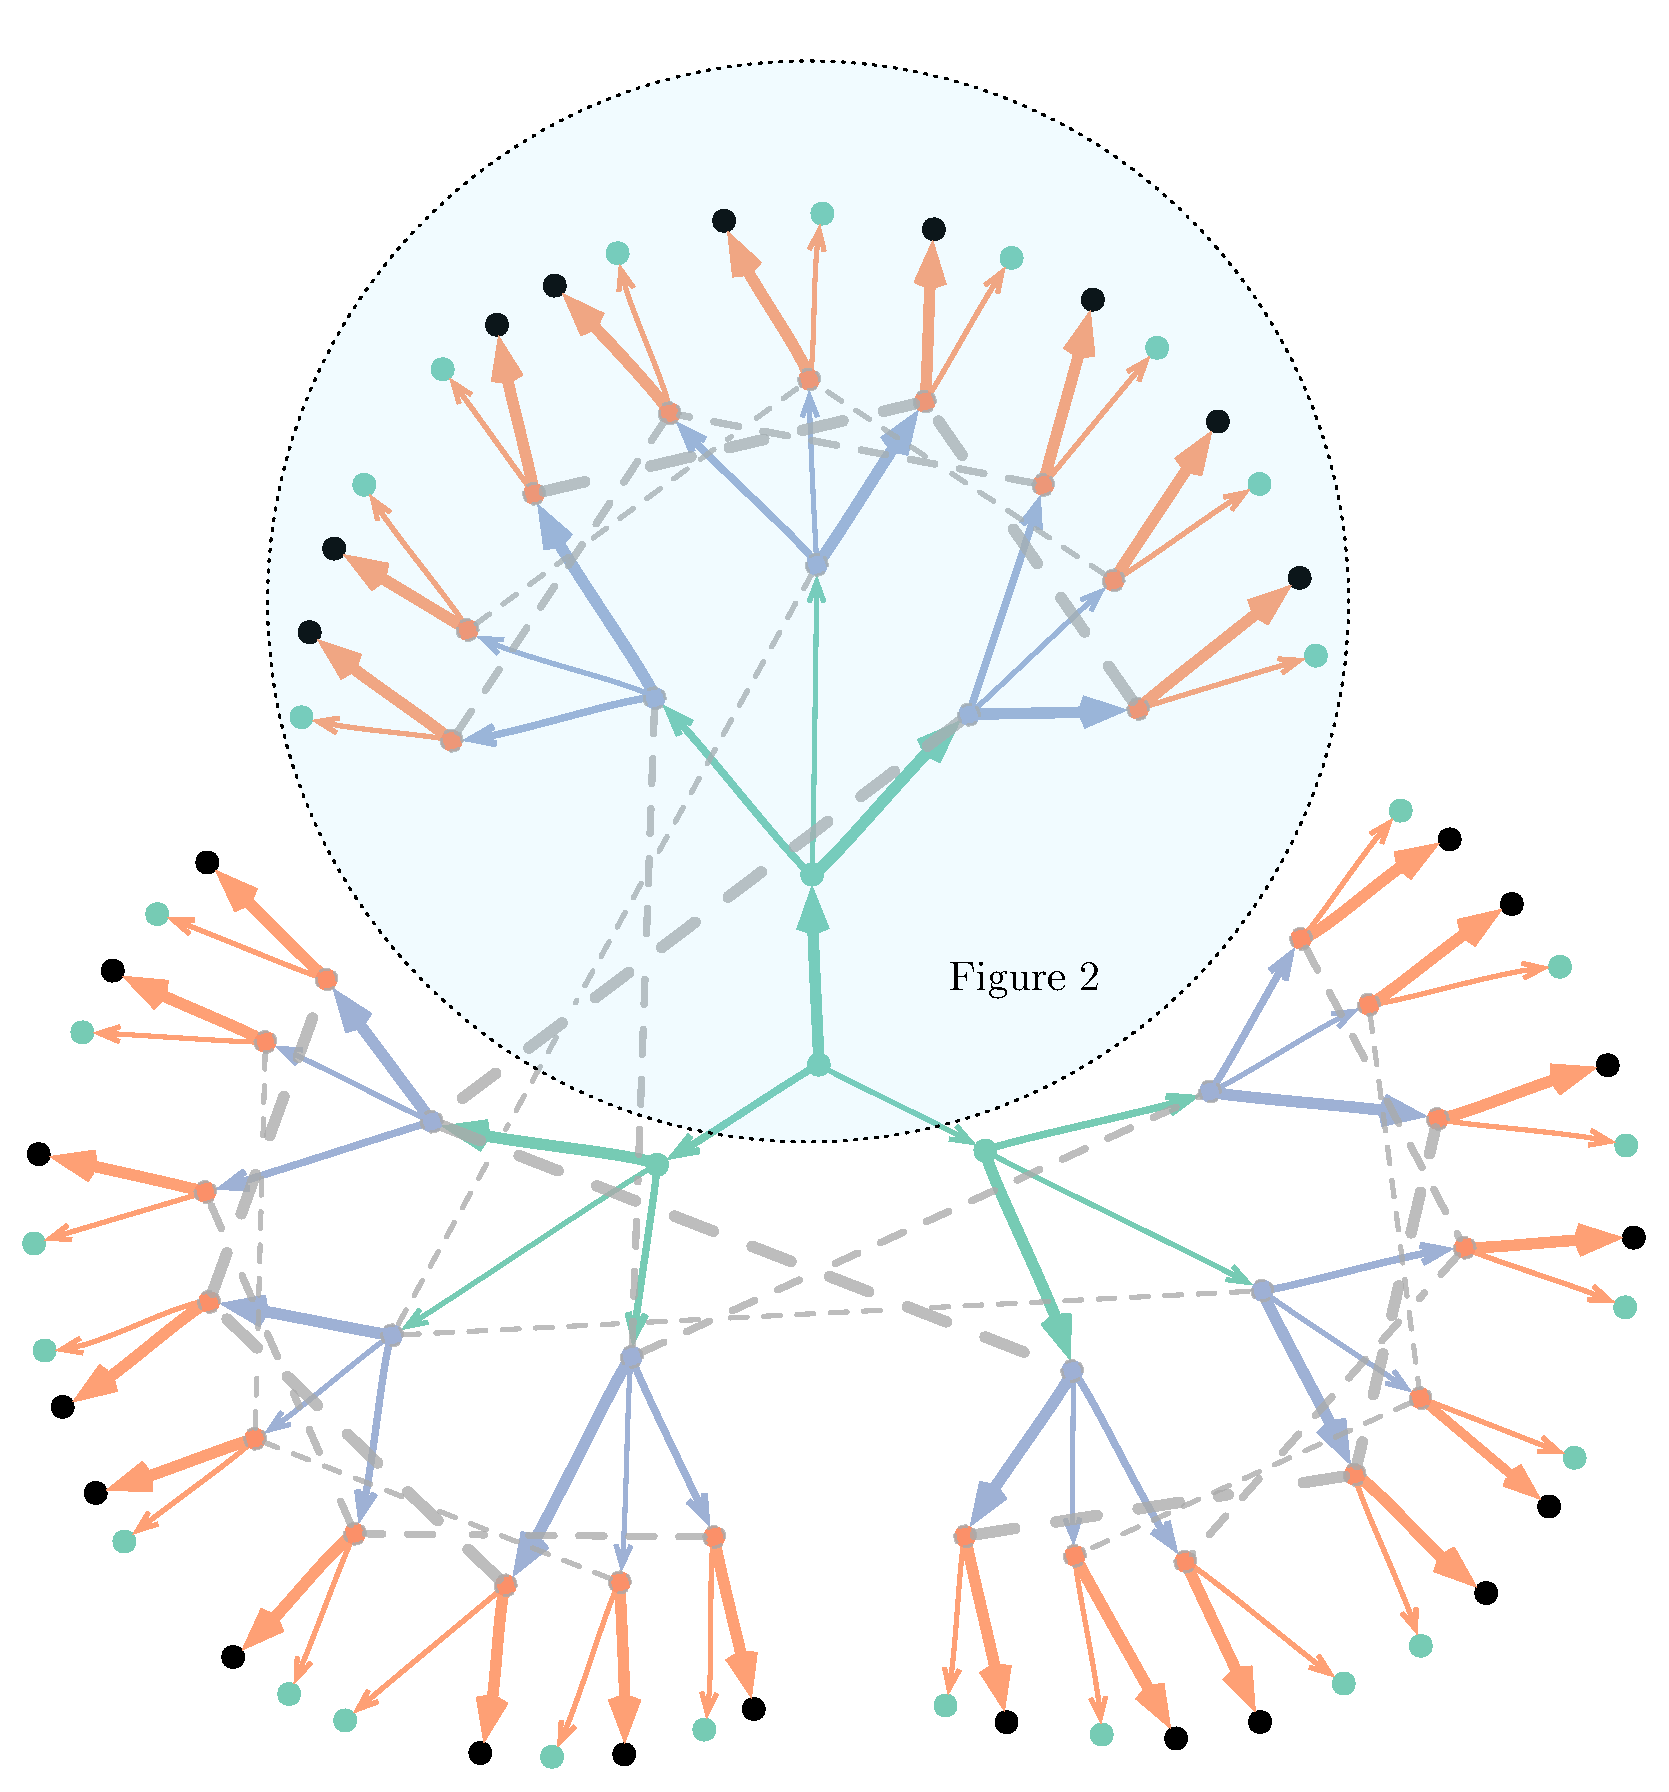
\includegraphics[width=119mm]{figures/rounded_clover_infosets}
\end{adjustbox}
\caption{Simplified game tree. Arrows correspond to two moves by nature, followed by women, and midwives respectively. Line weight distinguishes between information sets, and possible moves, corresponding to ascending player types. For midwives, referral is shown by a heavier arrow. Light terminal nodes indicate that the game may repeat from that point, and black nodes are exits}

\label{fig:simple_tree}
\end{figure}

\begin{figure}[H]
\begin{adjustbox}{center}
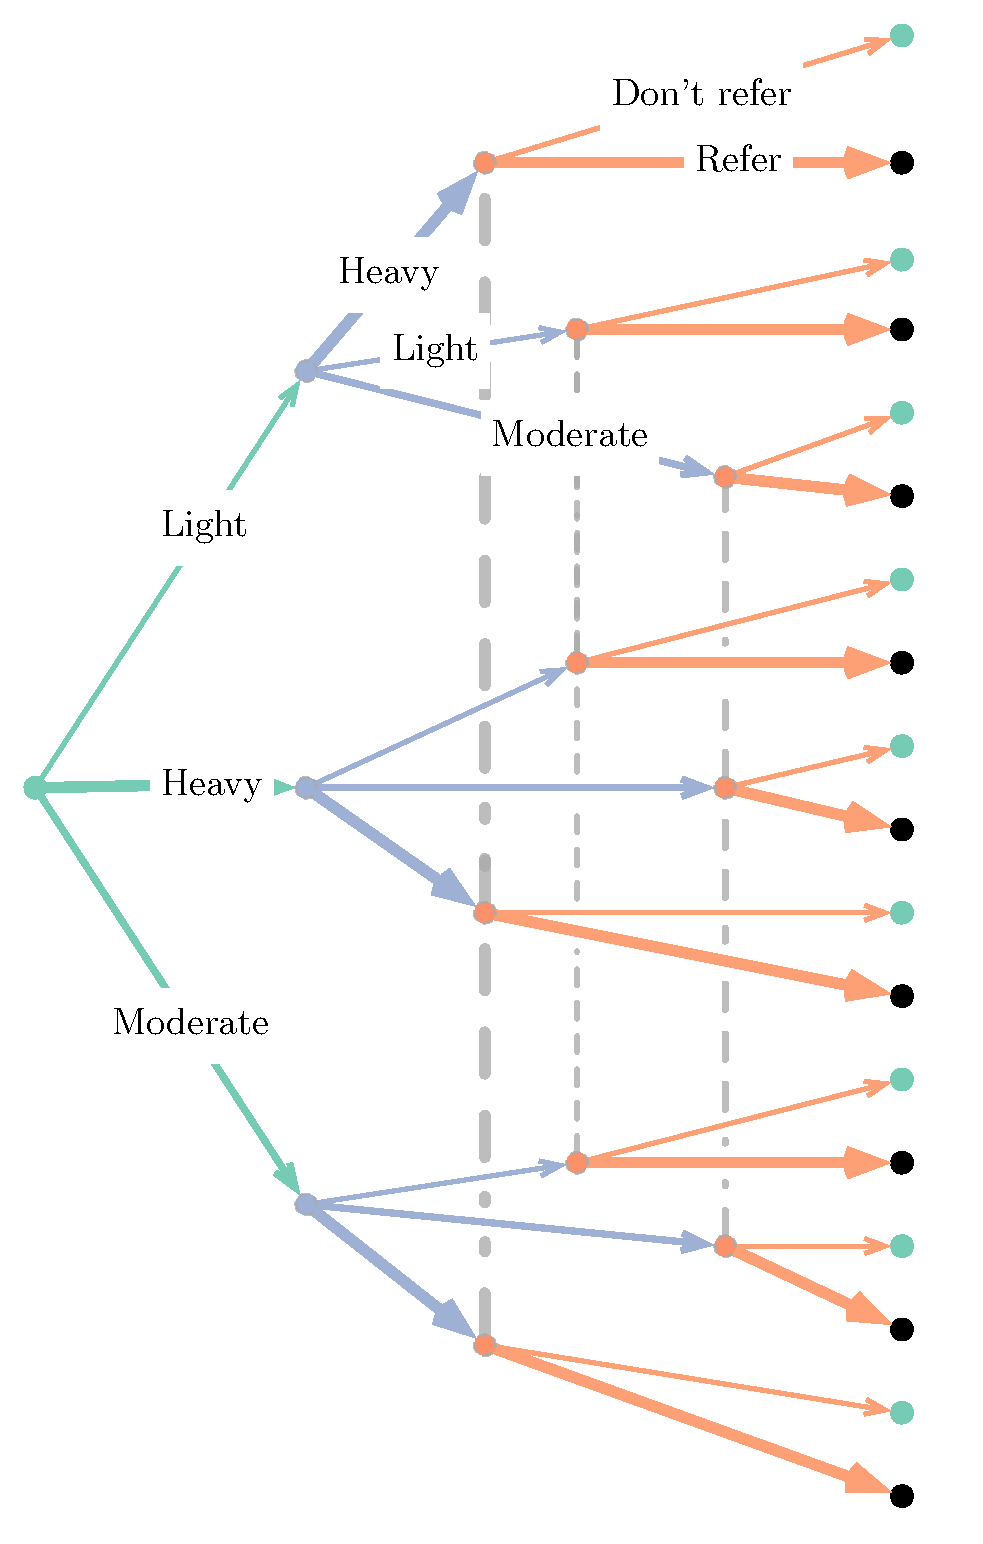
\includegraphics[width=119mm]{figures/tree_zoom}
\end{adjustbox}
\caption{Detail view of a single game tree branch, showing the possible moves by each player, with information sets for midwives}

\label{fig:zoom_tree}
\end{figure}

\begin{figure}[H]
\begin{adjustbox}{center}\subfloat[Women (heavy drinkers)]{\includegraphics[width=119mm]{figures/women_influence}}\end{adjustbox}
\vskip
\begin{adjustbox}{center}\subfloat[Midwives]{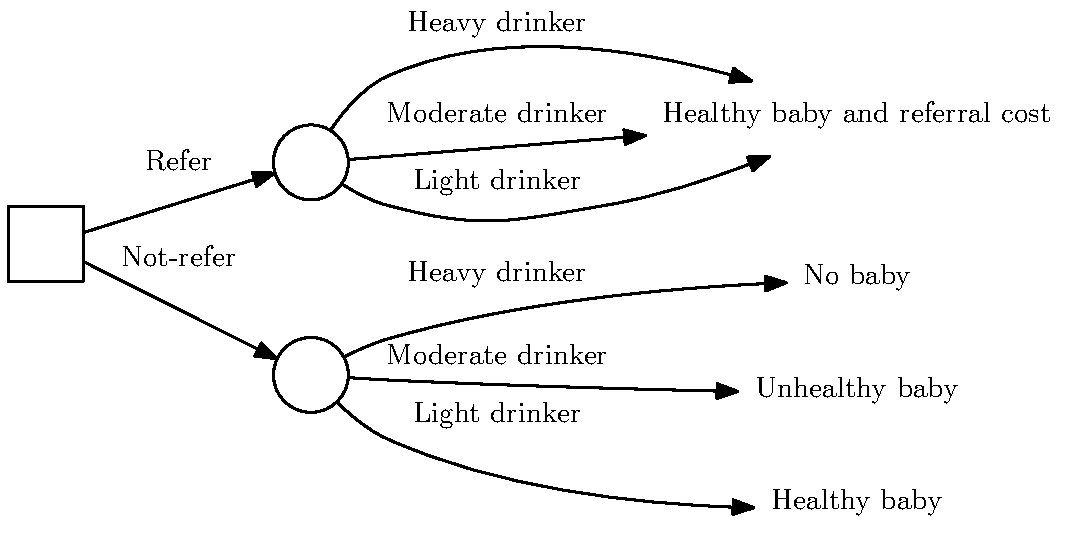
\includegraphics[width=119mm]{figures/mw_influence}}\end{adjustbox}
\caption{Influence diagrams, showing the game broken into two decision problems. Squares indicate a decision node, while circles are (from the perspective of the agent) chance nodes}

\label{fig:decision_problems}
\end{figure}

%Might belong in a more methody bit? Read some stuff to check..
To formally define the game, let \(N = \{m, w\}\) be the set of players each with a private type \(\theta_{i} \in \Theta\), and a set of types \(\Theta=\{l, m, h\}\), with pure strategies \(A_{m}=\{r,n\}, A_{w}=\{l, m, h\}\). Here, \(\{l, m, h\}\) correspond to light, moderate, and heavy alcohol consumption for women, and non-judgemental, moderately judgemental, and harshly judgemental for midwives. Midwives' pure strategies \(\{r,n\}\) are to refer, or do nothing, and those for women are to signal that they have one of the possible drinking patterns.
Additionally define two utility functions - 
\begin{equation}
u_{w}(s_{w}, s_{m}, \theta_{w}, \theta_{m})=X_{s, s_{w}, \theta_{m}} + X_{h, \theta_{w}, s_{m}}
\end{equation} 
\begin{equation}
u_{m}(s_{w}, s_{m}, \theta_{w})=X_{h, \theta_{w}, s_{m}} + X_{c, \theta_{w}, s_{m}},
\end{equation} with $X_{c}$, $X_{h}$, and $X_{s}$ being the payoff matrices as in table \ref{tab:Payoff-matrix}, $s_{w}$ and $s_{m}$ denoting a specific signal by a woman, and referral response by a midwife. Lastly let \(p_{w}(l, m, h)\), \(p_{m}(l, m, h)\) be distributions over types of women, and midwives respectively.


As noted, rather than solve the game, we allow populations of agents to play it, and hence stipulate further that women are drawn in order from a queue of \(n_{w}\) women (where \(n_{w}=1000\) in all simulations), and play against a midwife chosen at random from a population of \(n_{m}\) (\(n_{m}=100\)). They play for a maximum of \(r_{w}\) rounds (\(r_{w}=12\) following the routine number of ante-natal appointments in the UK \citep{NICE2010a}) or until they are referred, and a new player is drawn from the same distribution that produced the original players to replace them. If they are not referred, they rejoin the back of the queue after their appointment. In either case, they are informed of their payoff after each round and update their beliefs accordingly using one of the rules described in section \ref{sub:the_agents}.

Midwives play for \(r_{m}\) rounds (\(r_{m}=1000\) in all experiments), and conduct appointments in parallel, i.e. if there are 5 midwives, then five women are drawn from the queue and assigned at random to the midwives. 
Unlike women, midwives are only informed of their payoff if they choose to make a referral. Both groups of agents have perfect recall, and midwives are assumed to retrospectively update their observations if they make a referral after a number of appointments.



\subsection{Agent Models}
\label{sub:the_agents}
%Outline basic structure, then specifics on each one.
%This should probably go lexic -> bayes payoff -> bayes -> CPT in order
% of complexity.
%suggest there are added shells of complexity
%		mention the info sharing because homophilly
%			related - the enhancement to the bayes/cpt agents is that they personalise, as much as anything.
%		properly explain dirichlet priors
% How about comparing the decision problem representation for the agent types?

While in principle a wide variety of agent models are possible, given that decision rules operate on essentially the same information, and produce the same outputs, we limit ourselves here to four. The simplest is a lexicographic rule (1), in the spirit of a \ac{FFH} \citep{Gigerenzer2004} which uses only information about payoffs given actions; this is followed by a Bayesian risk minimisation rule (2) using the same information; a second Bayesian risk rule (3) which uses information about the underlying lottery; and a two-stage \ac{CPT} \citep{Hau2008} agent (4) which is identical to 3, but uses the \ac{CPT} decision rule from \cite{Tversky1992}. Hence, each successive decision model adds a layer of sophistication to the problem representation while retaining the same input-output characteristics.

As noted in section \ref{sub:the_game}, agents have perfect recall, and midwives recognise women if they repeatedly encounter them. While agents recall perfectly and make use of the new information for retrospective updates, all four agent models make decisions `as-if' they were always facing a new \enquote{opponent}.

A simplifying assumption is made that all midwives have just qualified after receiving identical training. As a result, they have homogeneous beliefs about  women and assume to some extent that they are honest.
Women are heterogeneous in their prior observations, which are assigned stochastically and constrained such that they have encountered each scenario possible for their type at least once, with exactly \(k\) encounters overall.


\subsubsection{Lexicographic Heuristic}
\label{sub:lexico}

The lexicographic heuristic (algorithm \ref{alg:lexico}) follows the form of that used in \cite{Hau2008}, and assumes a simplified problem representation, where an action is a choice between combined lotteries. Functionally, the heuristic maintains a count of the number of times that each action was followed by a payoff, and chooses the action which most commonly has the best payoff, i.e. one reason decision making. Where there is no clear best action, but one or more is evidently worse, a choice must be made as to whether to discard the poorer action; in this case we have elected to retain it.
This approach requires minimal computation, and does not assume that \(u_{i}\) is static, or known.

Women resolve this by approximating the utility function, as a function \(f(s_{w}, \sigma)\) on their choice of signal and an unknown distribution $\sigma$, which maps to \(u_{w}\) - i.e. \(s_{w}\) is a choice between simple lotteries. The algorithm maintains a count, \(n\), of the number of occurrences of each outcome given the choice from \(s_{w}\).

Midwives solve a slightly different problem with more information, where \(s_{w}\) is known, and \(s_{m}\) is the lottery choice - \(f(s_{w}, s_{m},\sigma)\). This is resolved by maintaining a separate count for each signal (i.e. \(n_{s_{w},s_{m}}\)), and otherwise following the same algorithm, presented below.

\begin{algorithm}
\begin{algorithmic}
\State n=1, action=none
\While{action is none}
\State Calculate the nth most common outcome following each action.
\State Sort actions by the value of the nth most common outcome.
\If{clear winner} \State action = best \EndIf
\State n = n + 1
\EndWhile
\State \Return action
\end{algorithmic}
\caption{Lexicographic heuristic\label{alg:lexico}}
\end{algorithm}

\subsubsection{Bayesian Payoff}

The Bayesian payoff agent uses the same subset of information as the lexicographic method, but updates beliefs on the link between actions and payoffs using the Bayes rule, and attempts to choose the action which minimises risk.

Given the discrete nature of actions and payoffs, coupled with a desire for tractability of the
simulation, the Dirichlet distribution is employed as a prior to represent these beliefs. The probability
density function takes the form -

\begin{equation}
D(\Theta|\alpha)=\frac{\Gamma(\sum_{i=1}^{k}\alpha_{i})}{\prod_{i=1}^{k}\Gamma(\alpha_{i})}\overset{k}{\underset{i=1}{\prod}\Theta_{i}^{\alpha_{i-1}}}
\end{equation}


where \(\alpha=\{\alpha_{1}\ldots\alpha_{k}\}\), \(k\) is the number
of signal-payoff pairs, \(\Theta=\{x_{1},\,\ldots,x_{k-\text{1}}\}\) all
more than zero and summing to less than 1, and \(\alpha_{i}\) is the 
pseudo-count of prior observations for a pair \(i\). 

The distribution is particularly convenient, in that to infer the
probability of a signal implying a payoff becomes
simply -

\begin{equation}
p(x=j|D,\alpha)=\frac{\alpha_{j}+n_{j}}{\sum_{j}(\alpha_{j}+n_{j})}\label{eq:posterior}
\end{equation}


Where \(n_{j}\) is simply the count of occurrences of signal-payoff pair \(j\), so
that the belief that a signal will lead to a payoff is the number
of times that pairing has been observed (including the pseudo-count),
over the total number of observations thus far. This makes computation
of beliefs fast and simple, since all that must be maintained is
a count of observations with no particular concern as to their order.
As before, midwives follow a similar pattern but maintain \(n_{s_{w}}\) independent counts of pairings between referral choice and payoff, updating their beliefs about the relationship between the choice to refer and payoff given the signal they have received.

Agents then choose the strategy $s_{i}$ to minimise risk $R_{i}$, which is simply defined as - 
\begin{equation}
R_{w}(s_{w}) = \sum_{x \in X} -xp(x | s_{w})
\end{equation}
\begin{equation}
R_{m}(s_{w}, s_{m}) = \sum_{x \in X} -xp(x | s_{w}\wedge s_{m}),
\end{equation}

where $X$ is the set of payoffs the agent has observed to follow $s_{i}$.

\subsubsection{Bayesian Risk Minimisation}

The second Bayesian agent augments the reasoning of the simple payoff model, making the stronger assumption that the utility function is static, and known. Women maintain two sets of beliefs, corresponding respectively to \(p_{m}\), and the probability of referral given signal choice. This leads to the risk function, minimised with respect to \(s_{w}\) -

\begin{equation}
R_{w}(s_{w}, \theta_{w}) = \sum_{i\in A_{m}}\sum_{j\in \Theta} -u_{w}(s_{w}, i, \theta_{w}, j)p(j)p(i | s_{w}),
\end{equation}

so that the risk of a signal is the sum of the products of all payoffs with the probabilities of their entailed midwife types and responses.

Midwives reasoning centres on determining the meaning of signals, since given the knowledge of what some signal \(s_{w}\) conveys about the true type of the sender, the payoff for an action is known. As such, their inference process is the same as for the simple Bayesian agent but over signal-type pairs, and they attempt to minimise the following risk function, minimised with respect to \(s_{m}\) -

\begin{equation}
R_{m}(s_{w}, s_{m}) = \sum_{i\in \Theta} -u_{w}(s_{w}, s_{m}, i)p(i | s_{w})
\end{equation}

\subsubsection{Descriptive Decision Theory}

The most complex decision rule used is \ac{CPT}, which attempts to reproduce a number of systematic deviations from rationality observed in humans. While \ac{CPT} has primarily been applied in the context of decisions from description, it has been modified to deal with decisions from experience by incorporating a first stage where probabilities are estimates from observations as in \cite{FoxCPT}. In this instance the Bayesian inference process fills the first stage role.

%Maybe cut this bit and make explanation richer?
Rather than the psychologically more interesting \ac{PT}, the \ac{CPT}
decision rule is used in this instance, because of the requirement
for women to evaluate the `prospects'\footnote{Where a prospect is a payoff-probability pair, with the set of prospects for an action defining the possible outcomes for it.} of more than two actions. \ac{CPT} uses transformed probabilities, underweighting
small probabilities, and overweighting large ones. This is intended to reflect the observed behaviour of humans, where sufficiently high likelihoods are treated as certain, and contrastingly low probabilities as impossible. The correct weighting function is subject to some debate, but here we have used that of \citet{Tversky1992}, which treats probabilities differently for gains (eqn \ref{eqn:cpt_p_pos}) and losses (eqn \ref{eqn:cpt_p_neg}) -

\begin{align}
w^{+}(p) & = & \frac{p^{\gamma}}{(p^{\gamma}+(1-p)^{\gamma})^{\frac{1}{\gamma}}}\label{eqn:cpt_p_pos}\\
w^{-}(p) & = & \frac{p^{\delta}}{(p^{\delta}+(1-p)^{\delta})^{\frac{1}{\delta}}}\label{eqn:cpt_p_neg},
\end{align}


where $p$ is the unweighted probability, and $\gamma$ and $\delta$
are the weights for gain and loss probabilities respectively. Along similar lines, the values of losses and gains are transformed to reflect a tendency to regard a loss as more significant than a gain  -

\begin{equation}
v(u_{i})=\begin{cases}
f(u_{i}),& \text{if}\, u_{i}>0\\
0,& \text{if}\, u_{i}=0\\
\lambda g(u_{i}),& \text{if}\, x<0
\end{cases},
\end{equation}


where,

\begin{equation}
f(u_{i})=\begin{cases}
u_{i}^{\alpha},& \text{if}\,\alpha>0\\
\ln(u_{i}),& \text{if}\,\alpha=0\\
1-(1+u_{i})^{\alpha},& \text{if}\,\alpha<0
\end{cases}
\end{equation}
\begin{equation}
g(u_{i})=\begin{cases}
-(-u_{i})^{\beta},& \text{if}\,\beta>0\\
-\ln(-u_{i}),& \text{if}\,\beta=0\\
(1-u_{i})^{\beta}-1,& \text{if}\,\beta<0
\end{cases},
\end{equation}


and $\alpha$, and $\beta$ are respectively the power of a gain,
and a loss, and \(\lambda\) is a multiplier giving the aversion to loss. The \ac{CPT} value of outcome $u_{i}$, occurring with probability \(p\) is $v(u_{i})w^{+}(p)$
if $u_{i}\geq0$, and $v(u_{i})w^{-}(p)$ otherwise. For any given action the \ac{CPT}
value is the sum of the value of the prospects of that action, as
in the Bayesian risk model, and the agent chooses the option which maximises this quantity.

\subsection{Information Sharing}
\label{sub:info_sharing}

It would seem unreasonable to suppose that neither party recounts their experiences to their peers, and to explore the impact of this we also modify the game to introduce a simple form of information sharing within agent groups. This takes the form of having each agent share their memories with their colleagues with some probability \(q\). Individuals then incorporate shared information into their beliefs using weighted updates, such that a shared observation of a low type signal contributes to their beliefs by \(w\), and \(0\leq w\leq 1\) (i.e. \(n_{j} = n_{j} + w\)).
Women share only when they have finished play, and provide their complete history of games, because they have accurate information about the outcomes. By the same rationale, midwives share only their history with the most recent woman they referred. Sharing occurs simultaneously for all players at the end of each round, and all memories are either shared immediately or discarded.\footnote{More precisely, memories of games remain, but it is assumed that only the most current information is relevant enough to be shared.}

Because of their differing problem representations, the simple payoff reasoners and their more complex counterparts incorporate this exogenous information differently. The simple payoff based rule relies on a belief structure relating actions directly to rewards which is essentially model free. Because payoffs differ by the agent's private type, the information shared may not correspond to the experience of the listening agent in the same scenario. As a result, payoff reasoners have a belief bias towards the most common player type, and can believe in outcomes that are, for them, impossible.

By contrast, representing the problem in terms of the probabilities of the individual lotteries imposes a model that abstracts the new information from payoffs, and allows the agent to discard implausible outcomes. This stronger assumption as to the static and known qualities of payoffs does however reduce the flexibility of the decision rule.

%!TEX root = disclosure_game.tex
\section{Method}
\label{sec:method}
%Lay out the design of experiments, harking back to things we're looking for
%from the real world.

This section provides details of experiments conducted to examine the ability of the model to reproduce qualitative trends reported in the midwifery literature by \cite{Alvik2006}, and \cite{Phillips2007}; as well as a global sensitivity analysis and construction of statistical emulators to explore, and contrast the response surfaces of the four decision rules.

\subsection{Qualitative Trends}
\label{sub:qt}
%explicit subsection on the SA.


Throughout this paper, parameters for the \ac{CPT} model were as used in \cite{Tversky1992} (table \ref{tab:qt_params}). While there has been significant work on determining appropriate parameterisation for the model (e.g. \cite{Neilson2002}, \cite{Glockner2012}, \cite{Nilsson2011}), a full exploration of the impact of these parameters, or heterogeneous values within populations is beyond the scope of this work.

Two key measures were used - the fraction of the subpopulation who had ever signalled honestly, and the proportion referred. Both measures were taken after every round of play, and were taken relative to the agent's position in their sequence of appointments giving the probability of signalling honestly, or being referred having had a given number of appointments.

\begin{table}
\center
\begin{tabular} {|l | c | r|}
\hline
Name & Description & Value \\ \hline
\(N_{w}\) & Number of women & 1000 \\ \hline
\(N_{m}\) & Number of midwives & 100 \\ \hline
\(A_{m}\) & Number of appointments per midwive & 1000 \\ \hline
\(A_{w}\) & Maximum number of appointments per woman & 12 \\ \hline
R & Runs & 1000 \\ \hline
\(P_{h,w}\) & Proportion of heavy drinkers & \(1/3\) \\ \hline
\(P_{m,w}\) & Proportion of moderate drinkers & \(1/3\) \\ \hline
\(P_{l,w}\) & Proportion of light drinkers & \(1/3\) \\ \hline
\(P_{h,m}\) & Proportion of harsh midwives & \(5/100\) \\ \hline
\(P_{m,m}\) & Proportion of moderate midwives & \(10/100\) \\ \hline
\(P_{l,m}\) & Proportion of non-judgemental midwives & \(85/100\) \\ \hline
\(p_{w}\) & Probability of women sharing & 0. \\ \hline
\(q_{w}\) & Weight of shared information for women & 0. \\ \hline
\(p_{m}\) & Probability of midwives sharing & 0. \\ \hline
\(q_{m}\) & Weight of shared information for midwives & 0. \\ \hline
\(s_{i}[a_{i}]\) & Psuedo-count favouring honesty & 10 \\ \hline
\end{tabular}
\caption[Table caption text]{Model parameters. \label{tab:qt_params}}
\end{table}
\subsection{Global Sensitivity Analysis}
\label{sub:sensitivity}
%Maxmin latin hypercube -> remember to cite the r package used.
%Will require some discussion of the gemsa technique at this point - can also cite Jason H for precedent!
 \cite{Bijak2013b}

Parameters for training were generated in R \citep{RTeam2014} using Latin Hypercube Sampling \citep{Carnell2012} over the space of inputs given in table \ref{tab:sa_params}, giving 10 free parameters. Initially a unit hypercube was generated, then the margins transformed appropriately to cover those regions where the inputs are not bounded between 0 and 1, and for proportions of agent types which necessarily sum to one across the three parameters. Given the limitation of 400 design points for the \ac{GEM-SA} software, we produced exactly that many parameter combinations and collected results for 100 runs of each. A fixed set of 100 random seeds was used, such that each parameter set was run once with each seed, for every decision rule.

To better capture the response characteristics for the model, we measure three outcome variables - (1) the interquartile range of the average signal sent by each type of agent in a run, (2) the average signal of moderate drinking agents in a run, and (3) the standard deviation of that average signal between simulation runs. Together these three metrics give an indication of how far women are separable by their signalling behaviour (1), the behaviour of the at risk drinking groups\footnote{Under most conditions, the behaviour of heavy drinkers tracks closely with their moderate counterparts.} (2), and finally the stability of the system in the face of the stochastic elements.

Measurements were taken at the end of 1000 rounds of play, and for 1 and 2, 400 results were selected covering the full hypercube with each chosen randomly from the runs for that design point. This approach, rather than averaging across runs, was taken to avoid obscuring the high degree of variability evident in the output of the payoff reasoning agents in some areas of the parameter space.

Twelve emulators were built, covering each of the three output on all four decision models. These emulators were used to conduct a probabalistic sensitivity analysis using \ac{GEM-SA} to assess the impact of parameters individually, and in combination.

\begin{table}
\center
\begin{tabular} {|l | l | l| l|}
\hline
Name & Description & Min & Max \\ \hline
\(P_{h,w}\) & Proportion of heavy drinkers & 0 & 1 \\ \hline
\(P_{m,w}\) & Proportion of moderate drinkers & 0 & 1 \\ \hline
\(P_{l,w}\) & Proportion of light drinkers & 0 & 1 \\ \hline
\(P_{h,m}\) & Proportion of harsh midwives & 0 & 1 \\ \hline
\(P_{m,m}\) & Proportion of moderate midwives & 0 & 1 \\ \hline
\(P_{l,m}\) & Proportion of non-judgemental midwives & 0 & 1 \\ \hline
\(p_{w}\) & Probability of women sharing & 0 & 1 \\ \hline
\(q_{w}\) & Weight of shared information for women & 0 & 1 \\ \hline
\(p_{m}\) & Probability of midwives sharing & 0 & 1 \\ \hline
\(q_{m}\) & Weight of shared information for midwives & 0 & 1 \\ \hline
\(Payoff_{baby}\) & Health payoff for healthy delivery & 1 & 100 \\ \hline
\(Payoff_{referral}\) & Cost for referral & \multicolumn{2}{l|}{\(-(Payoff_{baby} - 1)\)} \\ \hline
\(s_{i}[a_{i}]\) & Psuedo-count favouring honesty & 1 & 100 \\ \hline
\end{tabular}
\caption[Table caption text]{Parameter ranges. \label{tab:sa_params}}
\end{table}

\begin{table}
\center
\begin{tabular} {| l | l |}
Name & Description \\ \hline



\end{tabular}
\caption[Table caption text]{Output measures. \label{tab:sa_measures}}
\end{table}

%!TEX root = disclosure_game.tex
%Include the descent into chaos bit
\section{Results}
\label{sec:results}


\subsection{Qualitative Trends}
\label{sub:qt_results}

As shown in figure \ref{fig:honest_signals}, all four decision rules were able to reproduce both qualitative trends towards more disclosure as women experience more appointments \citep{Phillips2007}, and a greater tendency towards underreporting of consumption by heavier drinkers \citep{Alvik2006}.  
Trends for all four rules are broadly similar, exhibiting a gradual increase across appointments which subsequently levels off. This levelling can in part be explained by the referral results shown in figure \ref{fig:ref_plot}, which show that the majority of drinkers are referred, even with substantial concealment. 

\begin{figure}[H]
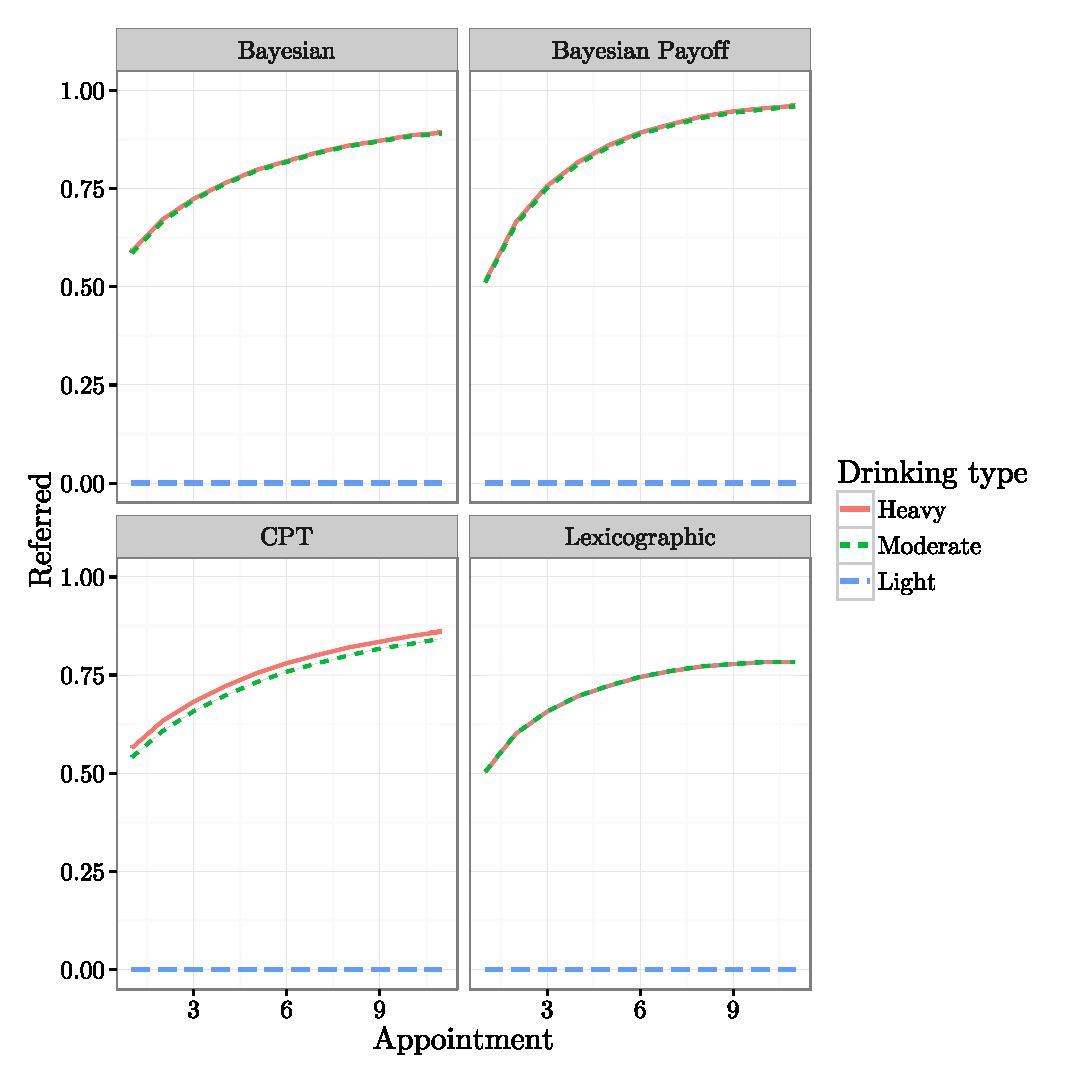
\includegraphics[width=100mm]{ref_plot}
\caption{Average fraction of population referred by each appointment, after 1000 rounds, mean with 95\% confidence limit over 1000 runs. Note that the large number of runs leads to very tight confidence intervals.\label{fig:ref_plot}}
\end{figure}

Referrals continue to occur, in the absence of honest signals, because drinkers are able to achieve a referral by masquerading as higher or lower types, dependent on how their initial beliefs are biased. Despite this the results suggest that a minority of risky drinkers will evade detection altogether, with no notable distinction between heavy and moderate types. Under these parameters, light drinkers always signal honestly and are never referred since there is no perceived advantage in doing so, and the evidence of deceptive signalling is insufficient to outweigh the biased priors of the midwives. 

\begin{figure}[H]
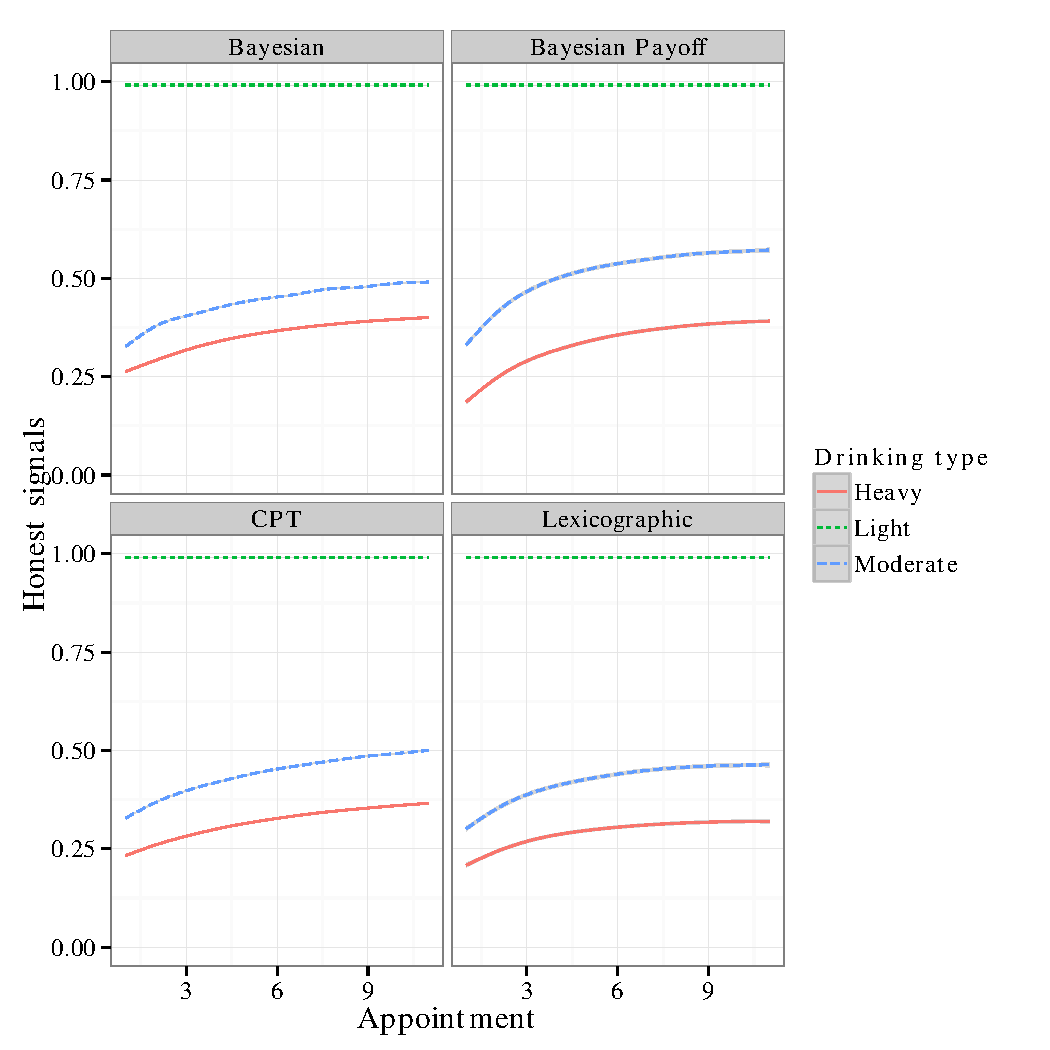
\includegraphics[width=100mm]{honesty_plot}
\caption{Average fraction of population ever signalled honestly by each appointment, after 1000 rounds, mean with 95\% confidence limit over 1000 runs. Note that the large number of runs leads to very tight confidence intervals.\label{fig:honest_signals}}
\end{figure}

\subsection{Social Learning}
\label{sub:sharing_results}

Introducing social learning amongst women leads the behaviour of the decision rules to diverge markedly, which we explore possible reasons for in section \ref{sec:discussion}. Figure \ref{fig:honest_sharing} shows the proportion of women who have signalled honestly at least once by their final appointment, under four sharing conditions. 

\begin{figure}[H]
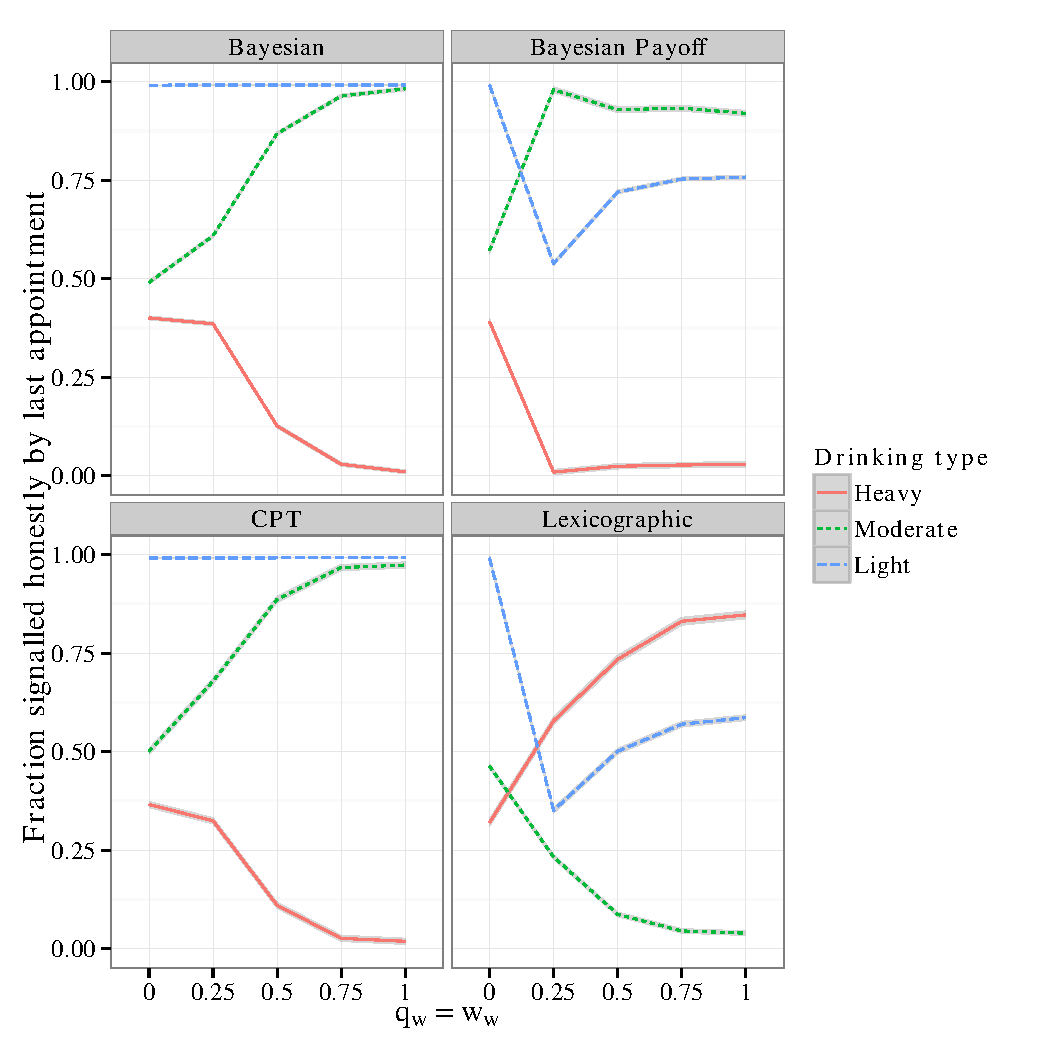
\includegraphics[width=100mm]{honesty_sharing}
\caption{Impact of social learning on trends in the average fraction of population ever signalled honestly by their final appointment, after 1000 rounds, mean with 95\% confidence interval over 100 runs}
\label{fig:honest_sharing}
\end{figure}

Aside from the lexicographic decision rule, the general tendency is towards less honest signalling by heavy drinkers, which is accompanied by a slight increase in referrals for the Bayesian, and \ac{CPT} rules. For these decision models, this is because social learning exacerbates the existing tendency of heavy drinkers to impersonate moderate drinkers, who behave more honestly as heavy drinkers become less so. This arises because both classes of agent learn that the moderate signal is the lower risk option as it is both a reliable indicator of need, and does not attract strongly negative judgement. The reliability of the signal is self reinforcing, since the more the agents use it and get referred, the more confident midwives become that it indicates need.

Particularly notable, is the decline in honest signalling by light drinkers visible in both heuristic type rules at the 0.25 level of \(q_{w}\) \& \(w_{w}\), which is associated with an increase in false positives. This arises because of the lack of homophily in social learning, as light drinkers become informed about negative outcomes associated with concealment, despite having nothing to conceal. The relatively high referral rates of drinkers heighten the effect further, because shared information becomes dominated by their experiences. 

The relationship is not, however, entirely straightforward, in that increasing social learning leads to greater variance between runs. A linear model was used to predict the between-runs interquartile range of the average signal sent by moderate drinkers. The predictors used were decision rule, and level of social learning, together with the interaction between the two. The regression results were significant (\(F_{7,12}=25,p<2.9\times10^{-6}\)) with \(R^2=94\%\), and intercept 0.07. The only significant coefficients were for the interaction terms, which were 0.44 (\(p<0.05\)) for the Bayesian payoff rule, and 0.69 (\(p<0.005\)) for the lexicographic. This suggests that social learning, for the heuristic style decision rules introduces considerable uncertainty to the model, which is explored further in the sensitivity analysis below.


\subsection{Sensitivity Analysis}
\label{sub:sa_results}

In this section we present a brief overview of the sensitivity analysis, followed by selected results highlighting the global effect of changes to perceived payoffs and degree of bias towards honesty, as well as social learning within women. The full results for the sensitivity analysis covering all sixteen emulators are available in appendix \ref{app:sensitivity_results}.

\begin{figure}[H]
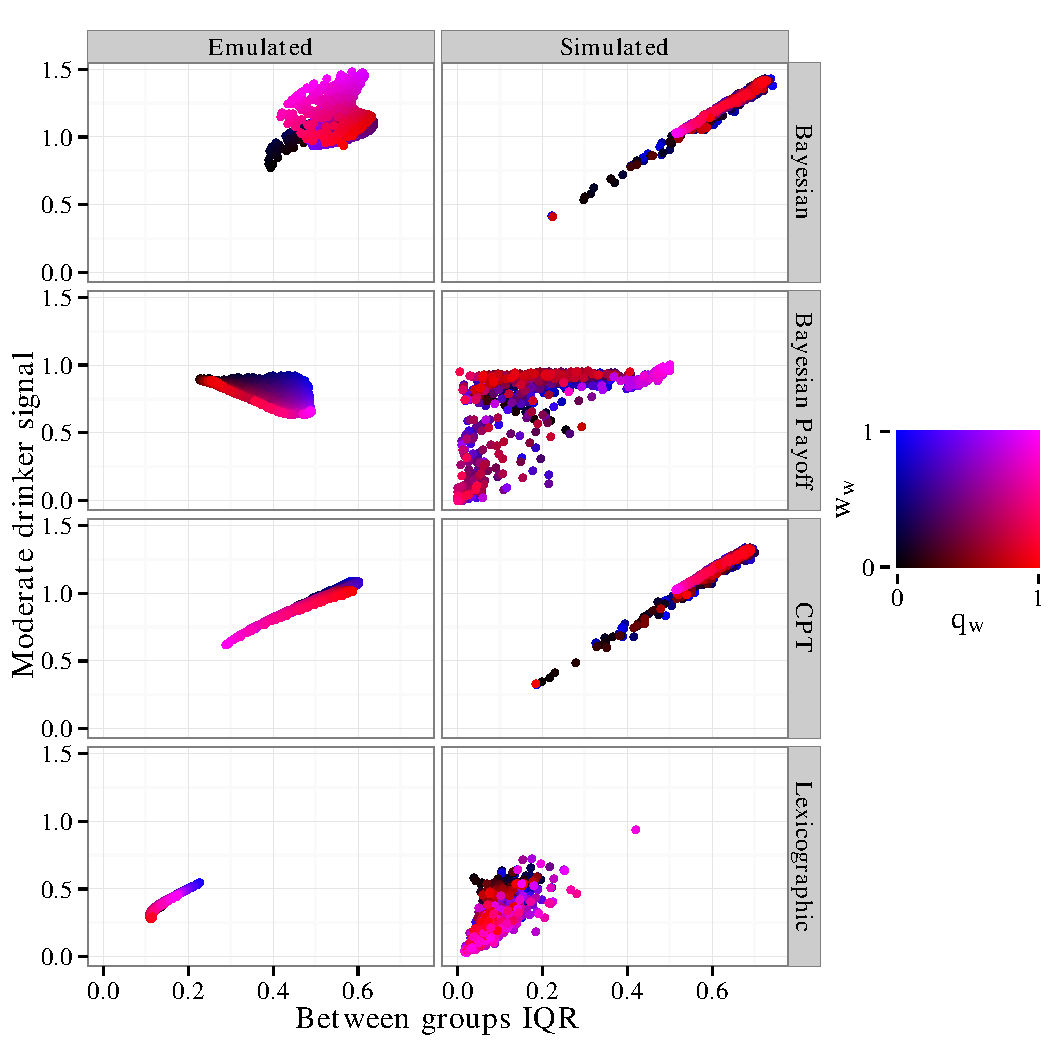
\includegraphics[width=90mm]{sharing_emulated_simulated}
\caption{Median moderate drinker signal vs median between drinking type IQR for all decision rules, with signals coded as 0 = light, 1 = moderate, and 2 = heavy.}
\label{fig:outcome_plots}
\end{figure}

For the median signal choice of moderate drinkers, the results of the sensitivity analysis suggest that the proportion of light drinkers has a significant effect for all decision rules, accounting for 10\%, 38\%, 24\%, and 5\% of the variance in output for the Lexicographic, Bayesian Payoff, Bayesian, and \ac{CPT} rules respectively. For the Lexicographic rule, the overwhelming majority of variance in signalling behaviour is reflective of the prevalence of stigmatisation by midwives (44\% \(p_{m}(m)\), 7\% \(p_{l}(m)\), and a further 15\% for their interaction).  The proportions of midwives are also key drivers in group separation, and the between run IQR of both measures for this rule. 

Perhaps surprisingly, variance attributable to social learning between midwives is relatively low, with neither the weight nor probability accounting for more than 5\% of variance in any measure. While there are small contributions to variance in interaction with other parameters (e.g. 4\% to between groups IQR, for the interaction with the proportion of light drinkers under the Bayesian rule), this may suggest that the model is lacking in this area, which we touch on in section \ref{sec:conclusion}.

Figure \ref{fig:outcome_plots} gives a qualitative picture of both emulator quality, and the divergent response surfaces of the decision rules in response to variations in social learning parameters. Emulator fit is clearly imperfect, but overall behaviour is qualitatively similar, with both emulated and simulated plots demonstrating separation in outcome space for the decision rules.

\begin{figure}[H]
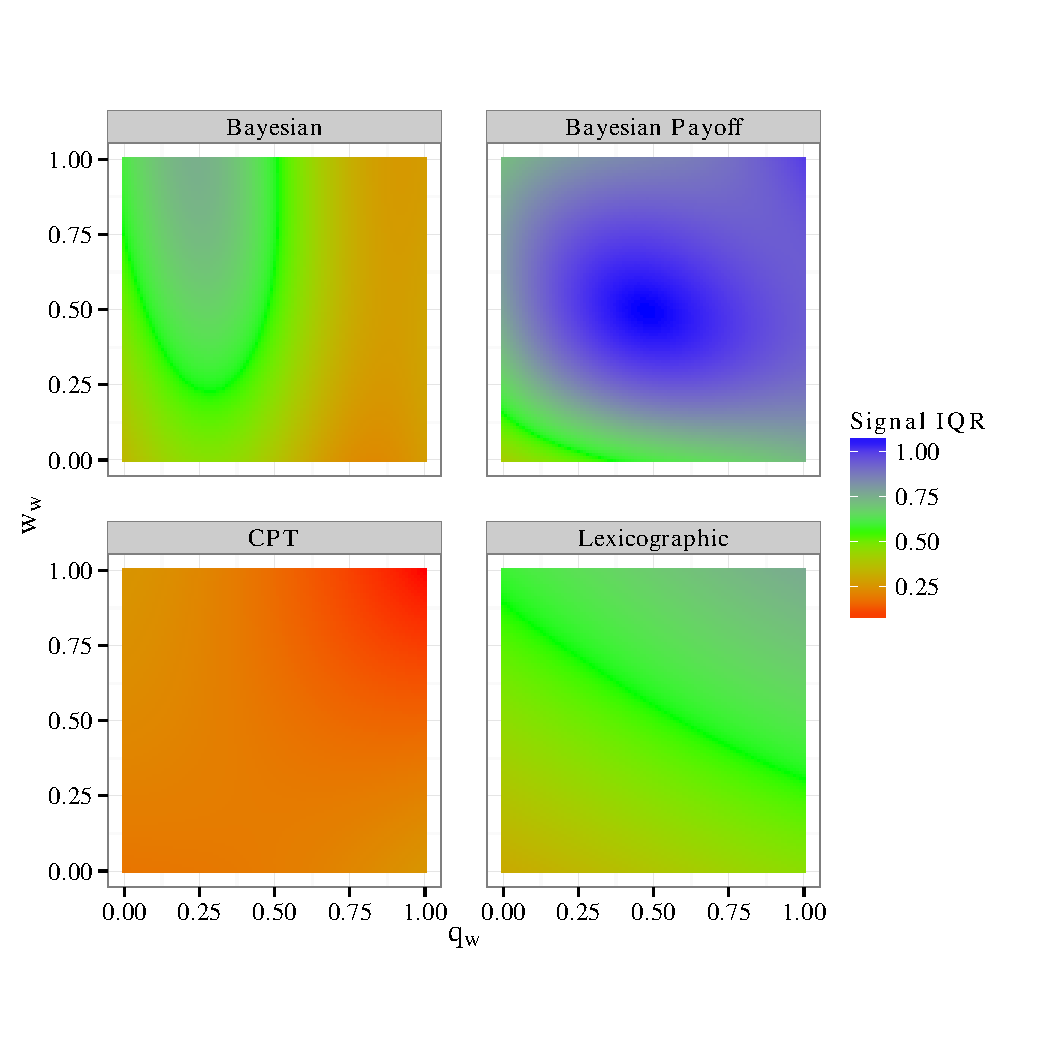
\includegraphics[width=100mm]{unfixed_emu_sig_iqr}
\caption{Emulated moderate drinker signal IQR in response to varying \(q_{w}\), and \(w_{w}\)}
\label{fig:emulated_sharing_iqr}
\end{figure}

Following from the suggestive results for social learning introducing uncertainty (section \ref{sub:sharing_results}), figure \ref{fig:emulated_sharing_iqr} shows emulated points covering the parameter space in high resolution. These plots reflect the increase in uncertainty of outcome shown for the heuristic type rules, which is especially severe for the Bayesian payoff rule. They also suggest that the Bayesian decision rule is less stable under conditions where the weight of shared information is substantially higher than the probability of sharing. This indicates that placing a high weight on information from limited sources leads to greater variability, i.e. what information is shared, matters.

\begin{figure}[H]
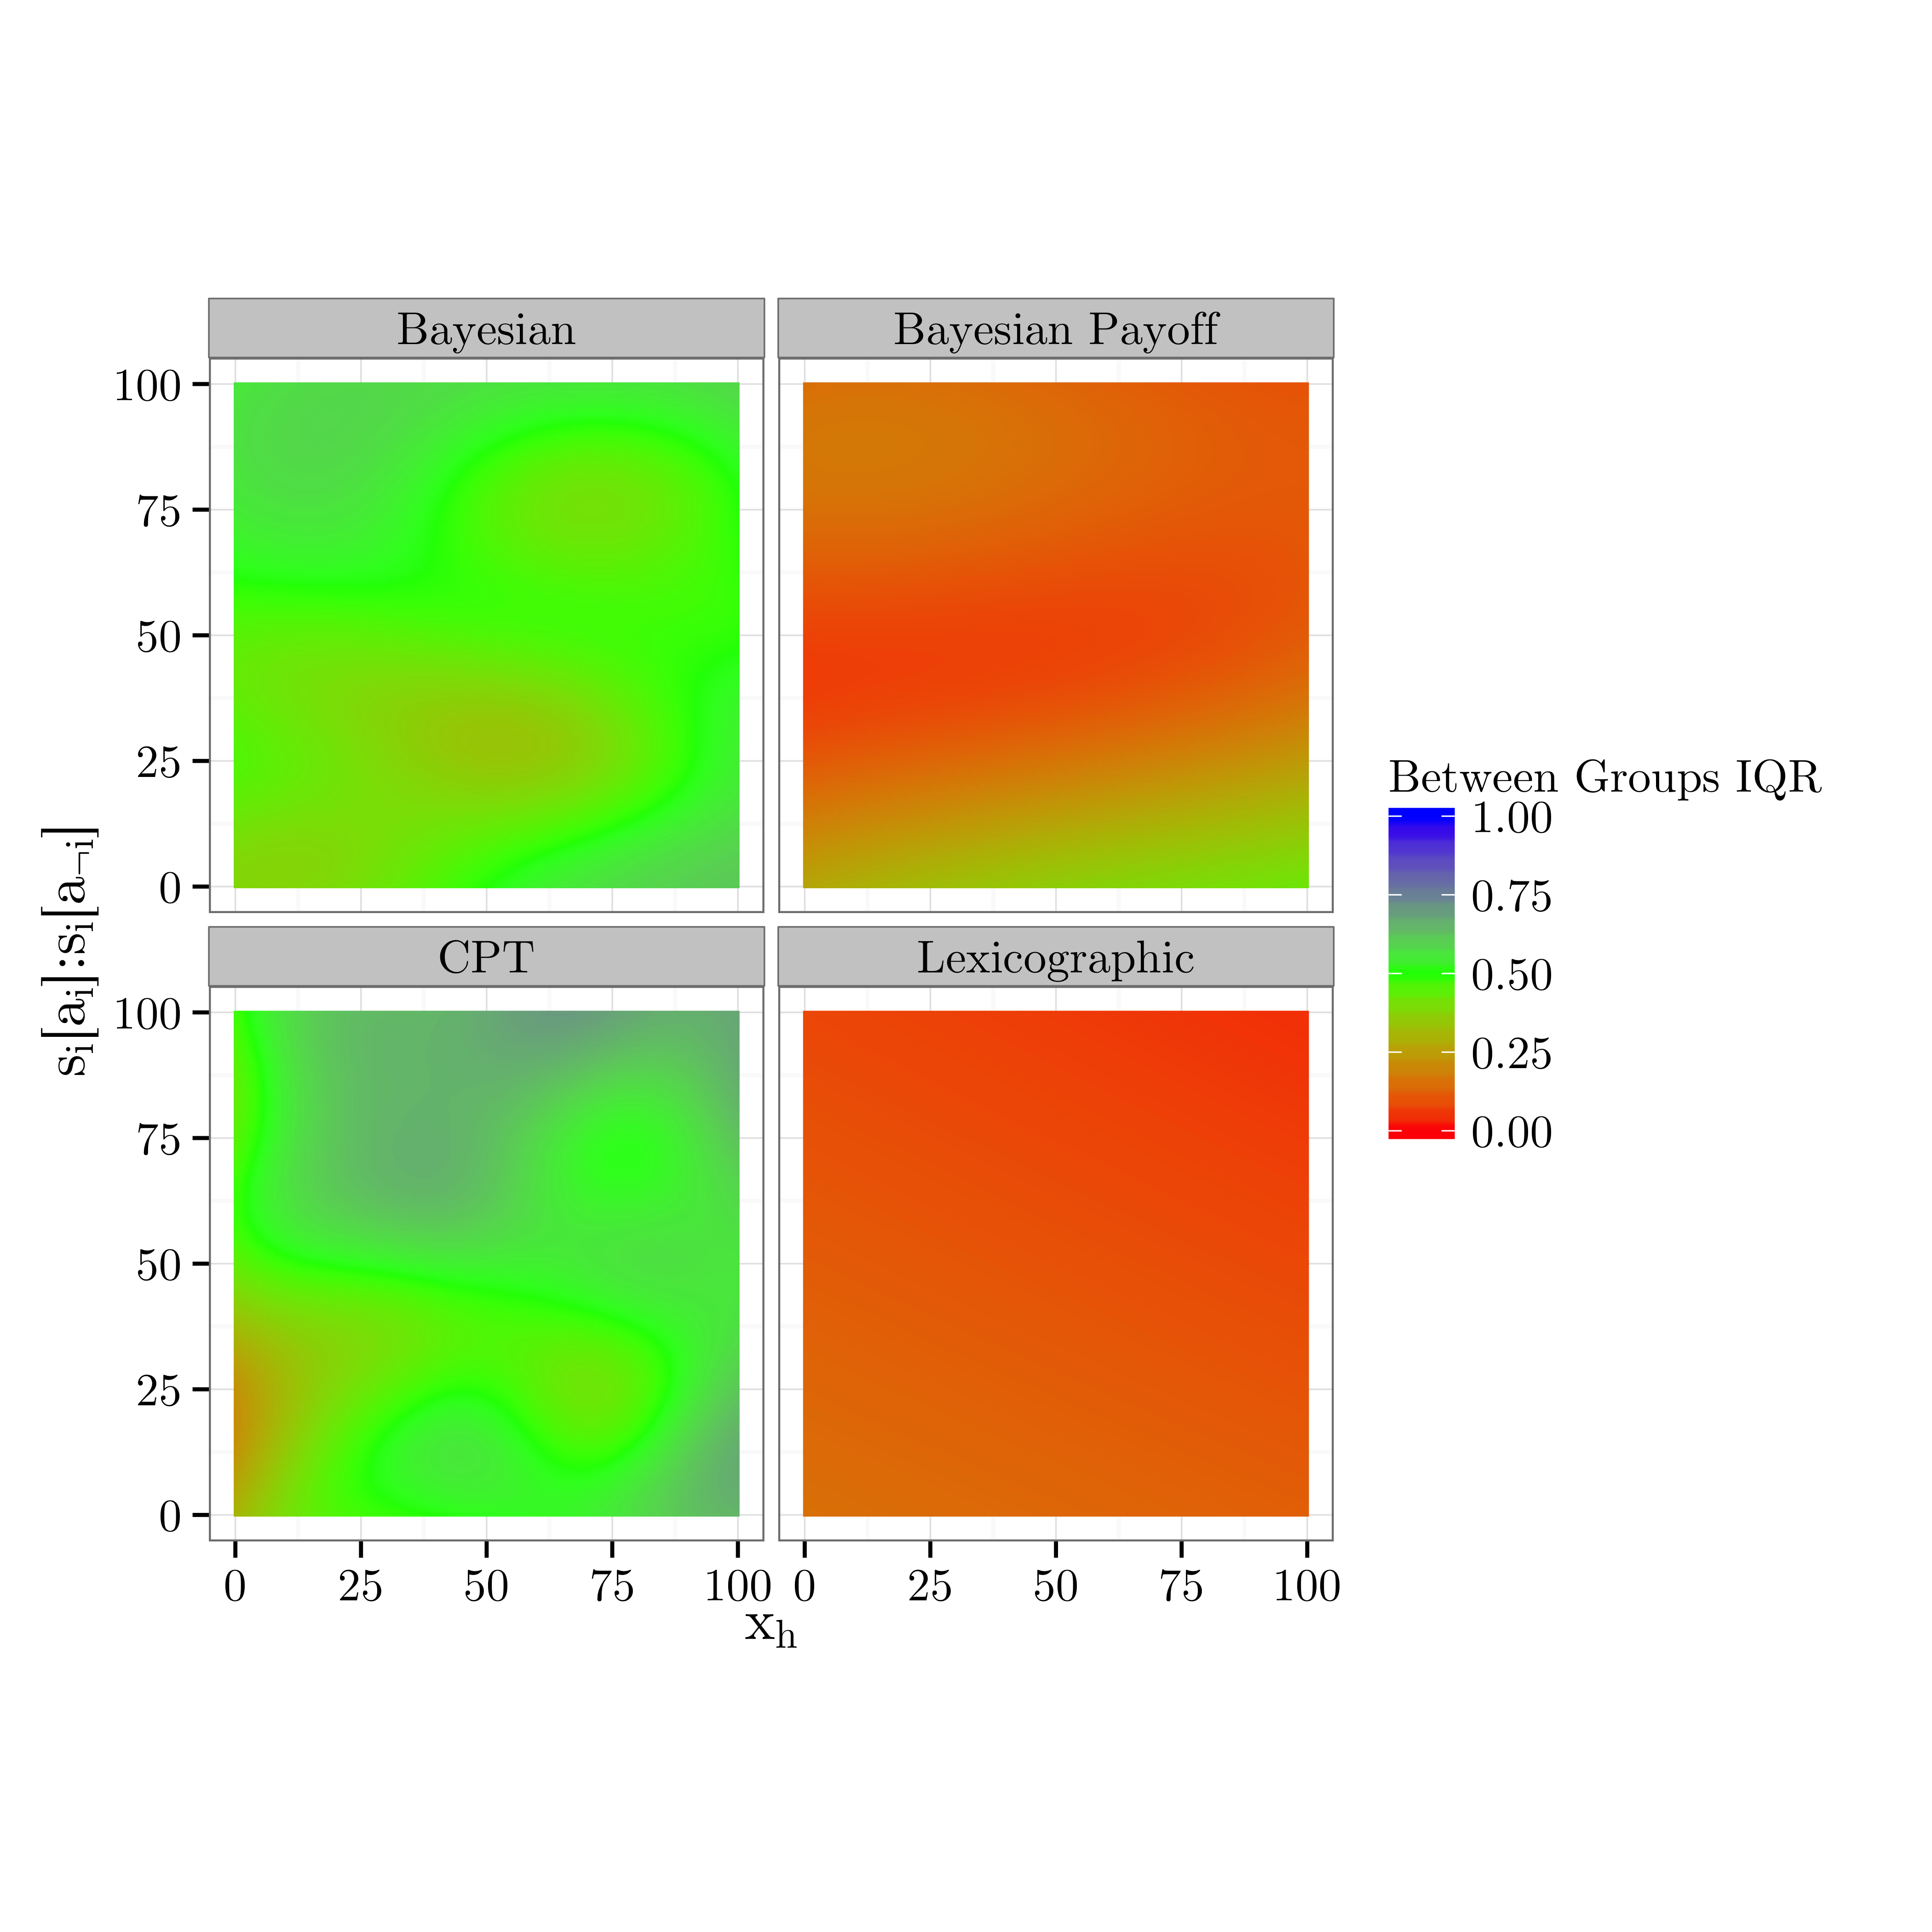
\includegraphics[width=100mm]{unfixed_emu_payoff_honesty_group_iqr}
\caption{Emulated between groups IQR in response to varying \(s_{i}[a_{i}]:s_{i}[a_{\neg i}]\), and \(x_{h}\)}
\label{fig:emulated_payoff_group_iqr}
\end{figure}

For the \ac{CPT}, and Bayesian decision models, the interaction of bias towards honesty, and distinction between payoffs has a significant, and non-linear effect on instability, and separability of groups. Figure \ref{fig:emulated_payoff_group_iqr} shows the effects, and also highlights the tendency towards poor separability of groups for both the heuristic type decision rules. The response surface of the Bayesian payoff rule is slightly more nuanced than the simple Lexicographic rule. Figure \ref{fig:emulated_payoff_group_iqr} shows better separation, close to partial pooling\footnote{Pooling occurs when signallers of different types `pool' their signals, and one adopts the signals of another.} at high payoff distinction, with relatively modest honesty bias, which is reflected by the variance contributions of 11\% and 8\% respectively.  For the more complex rules, the general tendency is towards less pooling for higher values of both, but with pockets where full pooling\footnote{Indicating that all signaller types are using a the same signal.} occurs.  The plots also suggest that the sensitivity of the \ac{CPT} rule is marginally greater, which is supported by the significant contribution to variance of close to 15\% for all measures of \(x_{h}\).


%!TEX root = disclosure_game.tex
\section{Discussion and Conclusions}
\label{sec:conclusion}
%reiterate contribution
%	bring up the simplicity -> chaos thing, talk about homophily
%	talk up the good (trends! yay!) and intro the bad -> no data
%
%	emphasise the 'nice story' -> future work
% ~ 1,500 words.

From a pragmatic perspective, the differing response characteristics of the decision rules are substantial and significant. The lack of a mechanism of homophily in the very simple rules leads to a high level of uncertainty in the overall dynamics, since even irrelevant information is taken at face value and to be equally valuable. By contrast, the belief structure of the \ac{CPT}, and Bayesian models represents a useful abstraction which allows the use of the relevant aspects of the information.  Naturally, incorporating homophily, by, for example weighting shared information by the type of the sharer, would represent a relatively trivial modification to the heuristic models. While to some extent this highlights the flexibility of the decision rule approach, it would of course sacrifice the parsimony of the model to a degree. This is an important consideration, given that part of the argument in favour of a decision theoretic approach to agent building lies in the minimal nature of the behavioural rules, which can be seen as occupying a middle ground between parameter and model.

One of the notable features of the results is the similarity in behaviour of the two classes of decision rule. To some extent this reflects poorly on the most complex rule, \ac{CPT}, which diverges only relatively minorly in behaviour from the Bayesian model. To some extent this might be anticipated, in that the payoffs are clearly unrealistic, which limits the utility of the \ac{CPT} approach.  Additionally, work by \citet{Glockner2012} has shown that there is considerable variation in individual parameters for the decision model, whereas we have let them remain homogenous here. In the vein, utility functions should arguably vary between individual agents, which could potentially be addressed by replacing the fixed payoffs used here with a distribution.  With this said, the significant increase in complexity, which entails both additional parameters and increases to simulation time may auger for a middle ground, particularly where elicitation of payoffs is impractical.  This, together with the variablility associated with the heuristic type decision rules speaks to a tradeoff between capturing reality, and replicating it.

Continuing the discussion of the issues raised by the representation of payoffs, the temporal aspect is significant, in that there is clearly a timing difference in payoffs, since while the potential social pain of disclosure is immediate, the health outcome comes only later. In light of this, that there is a known impact of time on perceived utility \citet{Thaler1981} suggests that incorporating some form of temporal discounting (e.g. exponential \citep{Samuelson1937}, or hyperbolic \citep{Ainslie1991}), or a decision model which explicitly treats intertemporal choice, such as the \ac{CPT} like model of \citet{Loewenstein1992}, is warranted. 

More broadly, the results demonstrate the logistical feasibility, and utility as a `tool for thinking', of an agent model grounded in decision theory. The results also make clear that deciding the operationalisation of the decision making is of key significance.

The conclusions that can be drawn about the behaviours of real life women, and their midwives, are necessarily limited by the paucity of data available to validate the model. While qualitative trends offer a some indication, they are clearly very limited in scope, and do not permit strong claims about the drivers of disclosure, and auger for a sceptical eye as to any recommendations targetted at improving outcomes.  With this said, the trends reported by \citet{Alvik2006}, and \citet{Phillips2007} are bourne out by the model, and predictions from the two more complex rules suggest that encouraging information sharing between women may encourage disclosure, but at the expense of reducing accuracy.

Further work will focus on applying the model to domains where validation data is more available, which will support a more comprehensive evaluation of the model discrepancy.  Disclosure is a widely applicable issue in health and social care and beyond, with examples ranging from a lack of help seeking behaviour noted in older men \citep{Smith2007a}, to the inverse scenario of innapropriate disclosure in social media \citep{christofides2009information}.
%!TEX root = disclosure_game.tex
\section*{Acknowledgements}
\label{sec:acknowledgements}

This work was supported by the Engineering and Physical Sciences Research Council 
(EPSRC) grant EP/H021698/1 Care Life Cycle, funded within the Complexity 
Science in the Real World theme. The authors also gratefully acknowledge the use of the IRIDIS High Performance Computing Facility, and associated support services at the University of Southampton, in the completion of this work.

\bibliography{library,library_addendum}
\bibliographystyle{spbasic}

\appendix
\setcounter{table}{0}
\renewcommand{\thetable}{A\arabic{table}}
%!TEX root = disclosure_game.tex
%Include the descent into chaos bit
\section{Sensitivity Analysis}
\label{app:sensitivity_results}

This section provides complete variance based sensitivity analysis results for the disclosure game model. Each subsection gives results for one simulation output under all four decision rules, with tables providing the percentage of overall variance attributable to the individual parameters, emulator quality statistics, and the 5 most significant interaction contributions to variance in the output.

\subsection{Median Moderate Drinker Signalling}

\begin{table}[H]
\caption{Median moderate drinker signalling parameter sensitivity \label{tab:sa_results_sig}}
\begin{tabular} {llllll}
\hline\noalign{\smallskip}
Parameter & Description & Lexicographic & Bayesian Payoff & Bayesian & \ac{CPT} \\
\noalign{\smallskip}\svhline\noalign{\smallskip}
\(p_{w}(m)\) & Proportion of moderate drinkers & 0.367 & 1.145 & 0.801 & 0.614 \\
\(p_{w}(l)\) & Proportion of light drinkers & 10.080 & 37.750 & 23.968  & 5.137\\
\(p_{m}(m)\) & Proportion of moderate midwives & 6.715 & 13.017 & 0.894 & 1.485\\
\(p_{m}(l)\) & Proportion of non-judgemental midwives & 43.942 & 1.655 & 1.602 & 2.618 \\
\(q_{w}\) & Probability of women sharing & 0.198 & 5.527 & 4.460 & 1.159 \\
\(w_{w}\) & Weight of shared information for women & 0.355 & 13.025 & 2.716 & 0.888 \\
\(q_{m}\) & Probability of midwives sharing & 0.145 & 0.667 & 0.368 & 0.157 \\
\(w_{m}\) & Weight of shared information for midwives & 0.118 & 0.376 & 0.176 & 0.200 \\
\(x_{h}\) & Health payoff for healthy delivery & 0.457 & 9.618 & 1.912 & 15.355 \\
\(s_{i}[a_{i}]:s_{i}[a_{\neg i}]\) & Pseudo-count favouring honesty & 0.140 & 7.537 & 10.427 & 7.795 \\
Total & All parameters and two way interactions & 86.777 & 96.527 & 85.529 & 74.123 \\
\noalign{\smallskip}\hline\noalign{\smallskip}
\end{tabular}
\end{table}

\begin{table}[H]
\caption{Median moderate drinker signalling emulator statistics \label{tab:sa_emulator_sig}}
\begin{tabular} {lllllll}
\hline\noalign{\smallskip}
Rule & \(\sigma^2\) & Nugget \(\sigma^2\) & Mean output & Total output variance & Code uncertainty & RMSSE \\
\noalign{\smallskip}\svhline\noalign{\smallskip}
Lexicographic & 0.834 & 0.131 &  0.817 & 0.012 & 0.252 & 1.746 \\
Bayesian Payoff & 1.667 & 0.475 &  0.662 & 0.003 & 0.181 & 3.12 \\
Bayesian & 3.352 & 0.534 & 1.160 & 0.001 & 0.068 & 2.423 \\
\ac{CPT} & 1.503 & 0.331 & 1.241 & 0.002 & 0.101 & 1.842 \\
\noalign{\smallskip}\hline\noalign{\smallskip}
\end{tabular}
\end{table}

\begin{table}[H]
\caption{Top 5 Interaction terms for \ac{CPT} decision rule. \label{tab:sa_interaction_prospect_sig}}
\begin{tabular} {ll}
\hline\noalign{\smallskip}
Parameter & Variance \\ 
\noalign{\smallskip}\svhline\noalign{\smallskip}

\(x_{h}\)*\(s_{i}[a_{i}]:s_{i}[a_{\neg i}]\) & 20.814\\
\(p_{w}(l)\)*\(s_{i}[a_{i}]:s_{i}[a_{\neg i}]\) & 5.698\\
\(p_{w}(l)\)*\(x_{h}\) & 2.895\\
\(s_{i}[a_{i}]:s_{i}[a_{\neg i}]\)*\(w_{w}\) & 2.799\\
\(s_{i}[a_{i}]:s_{i}[a_{\neg i}]\)*\(q_{m}\) & 1.686\\
\noalign{\smallskip}\hline\noalign{\smallskip}
\end{tabular}
\end{table}

\begin{table}[H]
\caption{Top 5 Interaction terms for Bayesian decision rule. \label{tab:sa_interaction_sharing_sig}}
\begin{tabular} {ll}
\hline\noalign{\smallskip}
Parameter & Variance \\
\noalign{\smallskip}\svhline\noalign{\smallskip}
\(p_{w}(l)\)*\(s_{i}[a_{i}]:s_{i}[a_{\neg i}]\) & 17.270\\
\(p_{w}(l)\)*\(q_{m}\) & 6.054\\
\(q_{m}\)*\(w_{w}\) & 3.814\\
\(s_{i}[a_{i}]:s_{i}[a_{\neg i}]\)*\(q_{m}\) & 3.538\\
\(s_{i}[a_{i}]:s_{i}[a_{\neg i}]\)*\(w_{w}\) & 3.084\\
\noalign{\smallskip}\hline\noalign{\smallskip}
\end{tabular}
\end{table}

\begin{table}[H]
\caption{Top 5 Interaction terms for Lexicographic decision rule. \label{tab:sa_interaction_lexic_sig}}
\begin{tabular} {ll}
\hline\noalign{\smallskip}
Parameter & Variance \\
\noalign{\smallskip}\svhline\noalign{\smallskip}
\(p_{m}(l)\)*\(p_{m}(m)\) & 15.331\\
\(p_{m}(m)\)*\(p_{w}(l)\) & 3.682\\
\(p_{m}(l)\)*\(p_{w}(l)\) & 3.581\\
\(p_{m}(m)\)*\(q_{m}\) & 0.349\\
\(p_{m}(l)\)*\(q_{m}\) & 0.279\\
\noalign{\smallskip}\hline\noalign{\smallskip}
\end{tabular}
\end{table}

\begin{table}[H]
\caption{Top 5 Interaction terms for Bayesian Payoff decision rule. \label{tab:sa_interaction_payoff_sig}}
\begin{tabular} {ll}
\hline\noalign{\smallskip}
Parameter & Variance \\
\noalign{\smallskip}\svhline\noalign{\smallskip}
\(p_{w}(l)\)*\(w_{w}\) & 4.045\\
\(x_{h}\)*\(s_{i}[a_{i}]:s_{i}[a_{\neg i}]\) & 1.856\\
\(p_{w}(l)\)*\(q_{m}\) & 1.231\\
\(s_{i}[a_{i}]:s_{i}[a_{\neg i}]\)*\(q_{m}\) & 0.997\\
\(q_{m}\)*\(w_{w}\) & 0.929\\ 
\noalign{\smallskip}\hline\noalign{\smallskip}
\end{tabular}
\end{table}



\subsection{Median Between Groups IQR}

\begin{table}[H]
\caption{Median between groups IQR parameter sensitivity \label{tab:sa_results_iqr}}
\begin{tabular} {llllll}
\hline\noalign{\smallskip}
Parameter & Description & Lexicographic & Bayesian Payoff & Bayesian & \ac{CPT} \\
\noalign{\smallskip}\svhline\noalign{\smallskip}
\(p_{w}(m)\) & Proportion of moderate drinkers & 0.327 & 0.688 & 0.457 & 0.586 \\
\(p_{w}(l)\) & Proportion of light drinkers & 11.223 & 20.123 & 11.046 & 4.081 \\
\(p_{m}(m)\) & Proportion of moderate midwives & 36.630 & 1.160 & 0.364 & 1.945 \\
\(p_{m}(l)\) & Proportion of non-judgemental midwives & 6.228 & 4.487 & 0.0964 & 2.627\\
\(q_{w}\) & Probability of women sharing & 0.498 & 0.235 & 2.537 & 1.812 \\
\(w_{w}\) & Weight of shared information for women & 1.018 & 2.307 & 1.889 & 0.740 \\
\(q_{m}\) & Probability of midwives sharing & 0.158 & 0.343 & 0.387 & 0.156 \\
\(w_{m}\) & Weight of shared information for midwives & 0.076 & 0.973 & 0.125 & 0.213 \\
\(x_{h}\) & Health payoff for healthy delivery & 0.317 & 10.960 & 3.305 & 16.493 \\
\(s_{i}[a_{i}]:s_{i}[a_{\neg i}]\) & Pseudo-count favouring honesty & 1.107 & 8.411 & 2.890 & 6.729 \\
Total & All parameters and two way interactions & 81.702 & 83.693 & 47.449 & 71.032 \\
\noalign{\smallskip}\hline\noalign{\smallskip}
\end{tabular}
\end{table}

\begin{table}[H]
\caption{Median between groups IQR emulator statistics \label{tab:sa_emulator_iqr}}
\begin{tabular} {lllllll}
\hline\noalign{\smallskip}
Rule & \(\sigma^2\) & Nugget \(\sigma^2\) & Mean output & Total output variance & Code uncertainty & RMSSE \\
\noalign{\smallskip}\svhline\noalign{\smallskip}
Lexicographic & 0.930 & 0.240 & 0.249 & 0.002 & 0.040 & 1.832 \\
Bayesian Payoff & 1.242 & 0.417 & 0.232 & 0.001 & 0.0034 & 2.308 \\
Bayesian & 1.254 & 0.131 & 0.644 & 0.000 & 0.019 & 1.167 \\
\ac{CPT} & 1.190 & 0.313 & 0.659 & 0.000 & 0.024 & 1.701 \\
\noalign{\smallskip}\hline\noalign{\smallskip}
\end{tabular}
\end{table}

\begin{table}[H]
\caption{Top five interaction terms for median between groups IQR \label{tab:sa_interaction_prospect_group_iqr}}
\begin{tabular} {lllll}
\hline\noalign{\smallskip}
Parameter & \multicolumn{4}{c}{Variance} \\ 
& \ac{CPT} & Bayesian & Lexicographic & \ac{PB} \\
\noalign{\smallskip}\svhline\noalign{\smallskip}

\(x_{h}\)*\(s_{i}[a_{i}]:s_{i}[a_{\neg i}]\) & 19.551 & 2.680&&2.360\\
\(p_{w}(l)\)*\(s_{i}[a_{i}]:s_{i}[a_{\neg i}]\) & 3.838 & 2.943 && 12.883\\
\(s_{i}[a_{i}]:s_{i}[a_{\neg i}]\)*\(w_{w}\) & 2.450\\
\(p_{w}(l)\)*\(x_{h}\) & 2.337 &&& 2.447\\
\(s_{i}[a_{i}]:s_{i}[a_{\neg i}]\)*\(q_{m}\) & 2.046 & 4.284\\
\(p_{w}(l)\)*\(q_{m}\) && 3.866\\
\(q_{m}\)*\(w_{w}\) && 2.282\\
\(p_{m}(l)\)*\(p_{m}(m)\) &&& 12.046\\
\(p_{m}(m)\)*\(p_{w}(l)\) &&& 5.054 & 1.919\\
\(p_{m}(l)\)*\(p_{w}(l)\) &&& 3.005\\
\(p_{m}(l)\)*\(w_{w}\) &&& 0.819\\
\(p_{m}(m)\)*\(w_{w}\) &&& 0.757\\
\(p_{w}(l)\)*\(w_{w}\) &&&& 5.667\\
\noalign{\smallskip}\hline\noalign{\smallskip}
\end{tabular}
\end{table}

\subsection{Median Moderate Drinker Signalling IQR}

\begin{table}[H]
\caption{IQR of median moderate drinker signalling parameter sensitivity \label{tab:sa_results_sig_iqr}}
\begin{tabular} {llllll}
\hline\noalign{\smallskip}
Parameter & Description & Lexicographic & Bayesian Payoff & Bayesian & \ac{CPT} \\
\noalign{\smallskip}\svhline\noalign{\smallskip}
\(p_{w}(m)\) & Proportion of moderate drinkers & 0.428 & 9.828 & 3.816 & 2.068 \\
\(p_{w}(l)\) & Proportion of light drinkers & 8.369 & 13.791 & 4.045 & 2.400 \\
\(p_{m}(m)\) & Proportion of moderate midwives & 13.416 & 0.712 & 0.676 & 0.583 \\
\(p_{m}(l)\) & Proportion of non-judgemental midwives & 21.079 & 0.648 & 0.659 & 0.373 \\
\(q_{w}\) & Probability of women sharing & 2.307 & 3.481 & 0.891 & 0.600 \\
\(w_{w}\) & Weight of shared information for women & 6.021 & 6.009 & 0.562 & 0.937 \\
\(q_{m}\) & Probability of midwives sharing & 0.315 & 1.829 & 0.114 & 0.117 \\
\(w_{m}\) & Weight of shared information for midwives & 1.652 & 1.354 & 0.260 & 0.0.139 \\
\(x_{h}\) & Health payoff for healthy delivery & 0.253 & 0.612 & 4.889 & 15.146 \\
\(s_{i}[a_{i}]:s_{i}[a_{\neg i}]\) & Pseudo-count favouring honesty & 0.504 & 3.096 & 19.863 & 25.999 \\
Total & All parameters and two way interactions & 84.9968 & 77.413 & 57.125 & 83.322 \\
\noalign{\smallskip}\hline\noalign{\smallskip}
\end{tabular}
\end{table}

\begin{table}[H]
\caption{IQR of median between groups IQR emulator statistics \label{tab:sa_emulator_sig_iqr}}
\begin{tabular} {lllllll}
\hline\noalign{\smallskip}
Rule & \(\sigma^2\) & Nugget \(\sigma^2\) & Mean output & Total output variance & Code uncertainty & RMSSE \\
\noalign{\smallskip}\svhline\noalign{\smallskip}
Lexicographic & 1.425 & 0.436 & 0.549 & 0.008 & 0.114 & 2.719 \\
Bayesian Payoff & 1.223 & 0.496 & 0.747 & 0.012 & 0.207 & 2.034 \\
Bayesian &  1.065 & 0.000 & 0.230 & 0.002 & 0.088 & 1.015 \\
\ac{CPT} & 0.874 & 0.213 & 0.233 & 0.001 & 0.066 & 1.806 \\
\noalign{\smallskip}\hline\noalign{\smallskip}
\end{tabular}
\end{table}

\begin{table}[H]
\caption{Top 5 Interaction terms for \ac{CPT} decision rule. \label{tab:sa_interaction_prospect_sig_iqr}}
\begin{tabular} {ll}
\hline\noalign{\smallskip}
Parameter & Variance \\ 
\noalign{\smallskip}\svhline\noalign{\smallskip}

\(x_{h}\)*\(s_{i}[a_{i}]:s_{i}[a_{\neg i}]\) & 17.377\\
\(p_{w}(m)\)*\(s_{i}[a_{i}]:s_{i}[a_{\neg i}]\) & 3.356\\
\(s_{i}[a_{i}]:s_{i}[a_{\neg i}]\)*\(w_{w}\) & 3.036\\
\(s_{i}[a_{i}]:s_{i}[a_{\neg i}]\)*\(q_{m}\) & 2.067\\
\(p_{w}(l)\)*\(s_{i}[a_{i}]:s_{i}[a_{\neg i}]\) & 1.721\\
\noalign{\smallskip}\hline\noalign{\smallskip}
\end{tabular}
\end{table}

\begin{table}[H]
\caption{Top 5 Interaction terms for Bayesian decision rule. \label{tab:sa_interaction_sharing_sig_iqr}}
\begin{tabular} {ll}
\hline\noalign{\smallskip}
Parameter & Variance \\
\noalign{\smallskip}\svhline\noalign{\smallskip}
\(p_{w}(m)\)*\(s_{i}[a_{i}]:s_{i}[a_{\neg i}]\) & 4.188\\
\(x_{h}\)*\(s_{i}[a_{i}]:s_{i}[a_{\neg i}]\) & 3.120\\
\(s_{i}[a_{i}]:s_{i}[a_{\neg i}]\)*\(q_{m}\) & 2.423\\
\(p_{w}(l)\)*\(s_{i}[a_{i}]:s_{i}[a_{\neg i}]\) & 2.279\\
\(p_{w}(l)\)*\(q_{m}\) & 1.489\\
\noalign{\smallskip}\hline\noalign{\smallskip}
\end{tabular}
\end{table}

\begin{table}[H]
\caption{Top 5 Interaction terms for Lexicographic decision rule. \label{tab:sa_interaction_lexic_sig_iqr}}
\begin{tabular} {ll}
\hline\noalign{\smallskip}
Parameter & Variance \\
\noalign{\smallskip}\svhline\noalign{\smallskip}
\(p_{m}(m)\)*\(p_{w}(l)\) & 12.068\\
\(p_{m}(l)\)*\(p_{w}(l)\) & 6.794\\
\(p_{m}(l)\)*\(p_{m}(m)\) & 5.567\\
\(p_{m}(m)\)*\(q_{m}\) & 0.886\\
\(p_{m}(l)\)*\(q_{m}\) & 0.692\\
\noalign{\smallskip}\hline\noalign{\smallskip}
\end{tabular}
\end{table}

\begin{table}[H]
\caption{Top 5 Interaction terms for Bayesian Payoff decision rule. \label{tab:sa_interaction_payoff_sig_iqr}}
\begin{tabular} {ll}
\hline\noalign{\smallskip}
Parameter & Variance \\
\noalign{\smallskip}\svhline\noalign{\smallskip}
\(p_{w}(l)\)*\(p_{w}(m)\) & 8.357\\
\(p_{w}(l)\)*\(w_{w}\) & 7.431\\
\(p_{w}(l)\)*\(s_{i}[a_{i}]:s_{i}[a_{\neg i}]\) & 4.882\\
\(p_{w}(l)\)*\(q_{m}\) & 2.346\\
\(p_{w}(l)\)*\(w_{m}\) & 2.025\\ 
\noalign{\smallskip}\hline\noalign{\smallskip}
\end{tabular}
\end{table}



\subsection{Between Groups IQR IQR}

\begin{table}[H]
\caption{IQR of median between groups IQR parameter sensitivity \label{tab:sa_results_iqr_iqr}}
\begin{tabular} {llllll}
\hline\noalign{\smallskip}
Parameter & Description & Lexicographic & Bayesian Payoff & Bayesian & \ac{CPT} \\
\noalign{\smallskip}\svhline\noalign{\smallskip}
\(p_{w}(m)\) & Proportion of moderate drinkers & 0.691 & 5.926 & 1.053 & 1.265 \\
\(p_{w}(l)\) & Proportion of light drinkers & 3.664 & 17.047 & 4.877 & 3.656 \\
\(p_{m}(m)\) & Proportion of moderate midwives & 41.369 & 1.124 & 0.814 & 0.591 \\
\(p_{m}(l)\) & Proportion of non-judgemental midwives & 7.109 & 0.739 & 0.496 & 0.378 \\
\(q_{w}\) & Probability of women sharing & 1.963 & 2.038 & 0.733 & 0.589 \\
\(w_{w}\) & Weight of shared information for women & 7.932 & 11.193 & 2.289 & 1.960 \\
\(q_{m}\) & Probability of midwives sharing & 0.413 & 1.972 & 0.267 & 0.069\\
\(w_{m}\) & Weight of shared information for midwives & 0.120 & 2.902 & 0.150 & 0.123 \\
\(x_{h}\) & Health payoff for healthy delivery & 0.228 & 3.190 & 6.308 & 14.777 \\
\(s_{i}[a_{i}]:s_{i}[a_{\neg i}]\) & Pseudo-count favouring honesty & 0.673 & 10.411 & 22.901 & 26.340 \\
Total & All parameters and two way interactions & 85.740 & 88.611 & 68.640 & 84.210 \\
\noalign{\smallskip}\hline\noalign{\smallskip}
\end{tabular}
\end{table}

\begin{table}[H]
\caption{IQR of median between groups IQR emulator statistics \label{tab:sa_emulator_iqr_iqr}}
\begin{tabular} {lllllll}
\hline\noalign{\smallskip}
Rule & \(\sigma^2\) & Nugget \(\sigma^2\) & Mean output & Total output variance & Code uncertainty & RMSSE \\
\noalign{\smallskip}\svhline\noalign{\smallskip}
Lexicographic & 0.826 & 0.409 & 0.259 & 0.002 & 0.034 & 2.364 \\
Bayesian Payoff & 3.202 & 0.520 & 0.328 & 0.002 & 0.032 & 2.452 \\
Bayesian & 1.177 & 0.041 & 0.133 & 0.000 & 0.018 & 1.152 \\
\ac{CPT} & 0.874 & 0.118 & 0.126 & 0.000 & 0.017 & 1.570 \\
\noalign{\smallskip}\hline\noalign{\smallskip}
\end{tabular}
\end{table}

\begin{table}[H]
\caption{Top 5 Interactions terms for \ac{CPT} decision rule. \label{tab:sa_interaction_prospect_group_iqr_iqr}}
\begin{tabular} {ll}
\hline\noalign{\smallskip}
Parameter & Variance \\ 
\noalign{\smallskip}\svhline\noalign{\smallskip}

\(x_{h}\)*\(s_{i}[a_{i}]:s_{i}[a_{\neg i}]\) & 18.626\\
\(p_{w}(l)\)*\(s_{i}[a_{i}]:s_{i}[a_{\neg i}]\) & 3.312\\
\(s_{i}[a_{i}]:s_{i}[a_{\neg i}]\)*\(w_{w}\) & 2.823\\
\(s_{i}[a_{i}]:s_{i}[a_{\neg i}]\)*\(q_{m}\) & 2.694\\
\(x_{h}\)*\(q_{m}\) & 1.022\\
\noalign{\smallskip}\hline\noalign{\smallskip}
\end{tabular}
\end{table}

\begin{table}[H]
\caption{Top 5 Interactions terms for Bayesian decision rule. \label{tab:sa_interaction_sharing_group_iqr_iqr}}
\begin{tabular} {ll}
\hline\noalign{\smallskip}
Parameter & Variance \\
\noalign{\smallskip}\svhline\noalign{\smallskip}
\(p_{w}(l)\)*\(s_{i}[a_{i}]:s_{i}[a_{\neg i}]\) & 7.947\\
\(x_{h}\)*\(s_{i}[a_{i}]:s_{i}[a_{\neg i}]\) & 4.048\\
\(s_{i}[a_{i}]:s_{i}[a_{\neg i}]\)*\(q_{m}\) & 3.134\\
\(p_{w}(l)\)*\(q_{m}\) & 2.307\\
\(p_{m}(m)\)*\(s_{i}[a_{i}]:s_{i}[a_{\neg i}]\) & 2.232\\
\noalign{\smallskip}\hline\noalign{\smallskip}
\end{tabular}
\end{table}

\begin{table}[H]
\caption{Top 5 Interactions terms for Lexicographic decision rule. \label{tab:sa_interaction_lexic_group_iqr_iqr}}
\begin{tabular} {ll}
\hline\noalign{\smallskip}
Parameter & Variance \\
\noalign{\smallskip}\svhline\noalign{\smallskip}
\(p_{m}(l)\)*\(p_{m}(m)\) & 8.659\\
\(p_{m}(m)\)*\(p_{w}(l)\) & 3.726\\
\(p_{m}(l)\)*\(p_{w}(l)\) & 3.237\\
\(p_{m}(l)\)*\(w_{w}\) & 1.564\\
\(p_{m}(m)\)*\(w_{w}\) & 1.558\\
\noalign{\smallskip}\hline\noalign{\smallskip}
\end{tabular}
\end{table}

\begin{table}[H]
\caption{Top 5 Interactions terms for Bayesian Payoff decision rule. \label{tab:sa_interaction_payoff_group_iqr_iqr}}
\begin{tabular} {ll}
\hline\noalign{\smallskip}
Parameter & Variance \\
\noalign{\smallskip}\svhline\noalign{\smallskip}
\(q_{m}\)*\(w_{w}\) & 3.830\\
\(p_{w}(l)\)*\(p_{w}(m)\) & 3.808\\
\(p_{w}(l)\)*\(s_{i}[a_{i}]:s_{i}[a_{\neg i}]\) & 3.401\\
\(p_{w}(l)\)*\(q_{m}\) & 2.385\\
\(x_{h}\)*\(s_{i}[a_{i}]:s_{i}[a_{\neg i}]\) & 2.294\\ 
\noalign{\smallskip}\hline\noalign{\smallskip}
\end{tabular}
\end{table}


\end{document}